\chapter{Pesquisa em memória externa}
\chaplabel{btree}

Ao longo deste livro, temos usado o modelo de computação com uma palavra de RAM de #w#-bits definido em \secref{model}. Uma suposição implícita desse modelo é que nosso computador tem uma memória de acesso aleatório grande o suficiente para armazenar todos os dados na estrutura de dados. Em algumas situações, essa suposição não é válida. Existem coleções de dados tão grandes que nenhum computador tem memória suficiente para armazená-los. Nesses casos, a aplicação deve recorrer ao armazenamento dos dados em algum meio de armazenamento externo, como um disco rígido, um disco de estado sólido ou mesmo um servidor de arquivos de rede (que possui seu próprio armazenamento externo).

\index{armazenamento externo}%
\index{memória externa}%
\index{disco rígido}%
\index{disco de estado sólido}%
O acesso a um item de armazenamento externo é extremamente lento. O disco rígido conectado ao computador no qual este livro foi escrito tem um tempo médio de acesso de 19ms e a unidade de estado sólido conectada ao computador tem um tempo médio de acesso de 0,3ms. Em contraste, a memória de acesso aleatório do computador tem um tempo médio de acesso inferior a 0,000113ms. O acesso à RAM é mais de 2.500 vezes mais rápido do que acessar a unidade de estado sólido e mais de 160.000 vezes mais rápido do que acessar o disco rígido.

%  HDD: Fantom ST3000DM001-9YN166 USB 3 external drive (3TB)
%  SSD: ATA OCZ-AGILITY 3 (60GB)
%  Mem: Mushkin Enhanced Essentials 4GB (2 x 2GB) 204-Pin DDR3 
%       SO-DIMM DDR3 1066 (PC3 8500) Dual Channel Kit Laptop Memory
%       Model 996643
%  RAM speed was estimated using this program:
% Xinclude<stdlib.h>
% Xinclude<stdio.h>
% Xinclude<time.h>
% 
% int main(void) {
%    unsigned *a, x, i, n = 50000000;
%    clock_t start, stop;
% 
%    start = clock();
%    a = malloc(sizeof(unsigned)*n);
%    for(i = 0; i < n; i++) {
%      x |= a[rand()%n];
%    }
%    stop = clock();
%    printf("x=%x, %g\n", x, (((double)(stop-start))/(double)CLOCKS_PER_SEC)/(double)n);
%    free(a);
%    return 0;
% }

Essas velocidades são bastante típicas; acessar um byte aleatório da RAM é milhares de vezes mais rápido do que acessar um byte aleatório de um disco rígido ou unidade de estado sólido. O tempo de acesso, entretanto, não conta toda a história. Quando acessamos um byte de um disco rígido ou disco de estado sólido, um \emph{bloco} inteiro
\index{bloco}%
do disco é lido.  Cada uma das unidades conectadas ao computador possui um tamanho de bloco de 4096; cada vez que lemos um byte, o drive nos dá um bloco contendo 4096 bytes. Se organizarmos nossa estrutura de dados com cuidado, isso significa que cada acesso ao disco pode render 4096 bytes que são úteis para completar qualquer operação que estivermos fazendo.

% morin@peewee:~/git/ods/latex$ sudo blockdev --report
% RO    RA   SSZ   BSZ   StartSec            Size   Device
% rw   256   512  4096          0     60022480896   /dev/sda   SSD
% rw   256  4096  4096        504   3000581885952   /dev/sdb1  HDD

Esta é a ideia por trás do \emph{modelo de memória externa}
\index{modelo de memória externa}%
de computação,
ilustrado esquematicamente em \figref{em}. Nesse modelo, o computador tem acesso a uma grande memória externa na qual residem todos os dados.
Esta memória é dividida em \emph{blocos} de memória 
\index{bloco}%
cada um contendo $B$
palavras.  O computador também possui memória interna limitada, na qual pode realizar cálculos. Transferir um bloco entre a memória interna e a memória externa leva um tempo constante. Os cálculos realizados na memória interna são \emph{gratuitos}; eles não levam tempo algum. O fato de os cálculos da memória interna serem gratuitos pode parecer um pouco estranho, mas simplesmente enfatiza o fato de que a memória externa é muito mais lenta do que a RAM.

\begin{figure}
  \centering{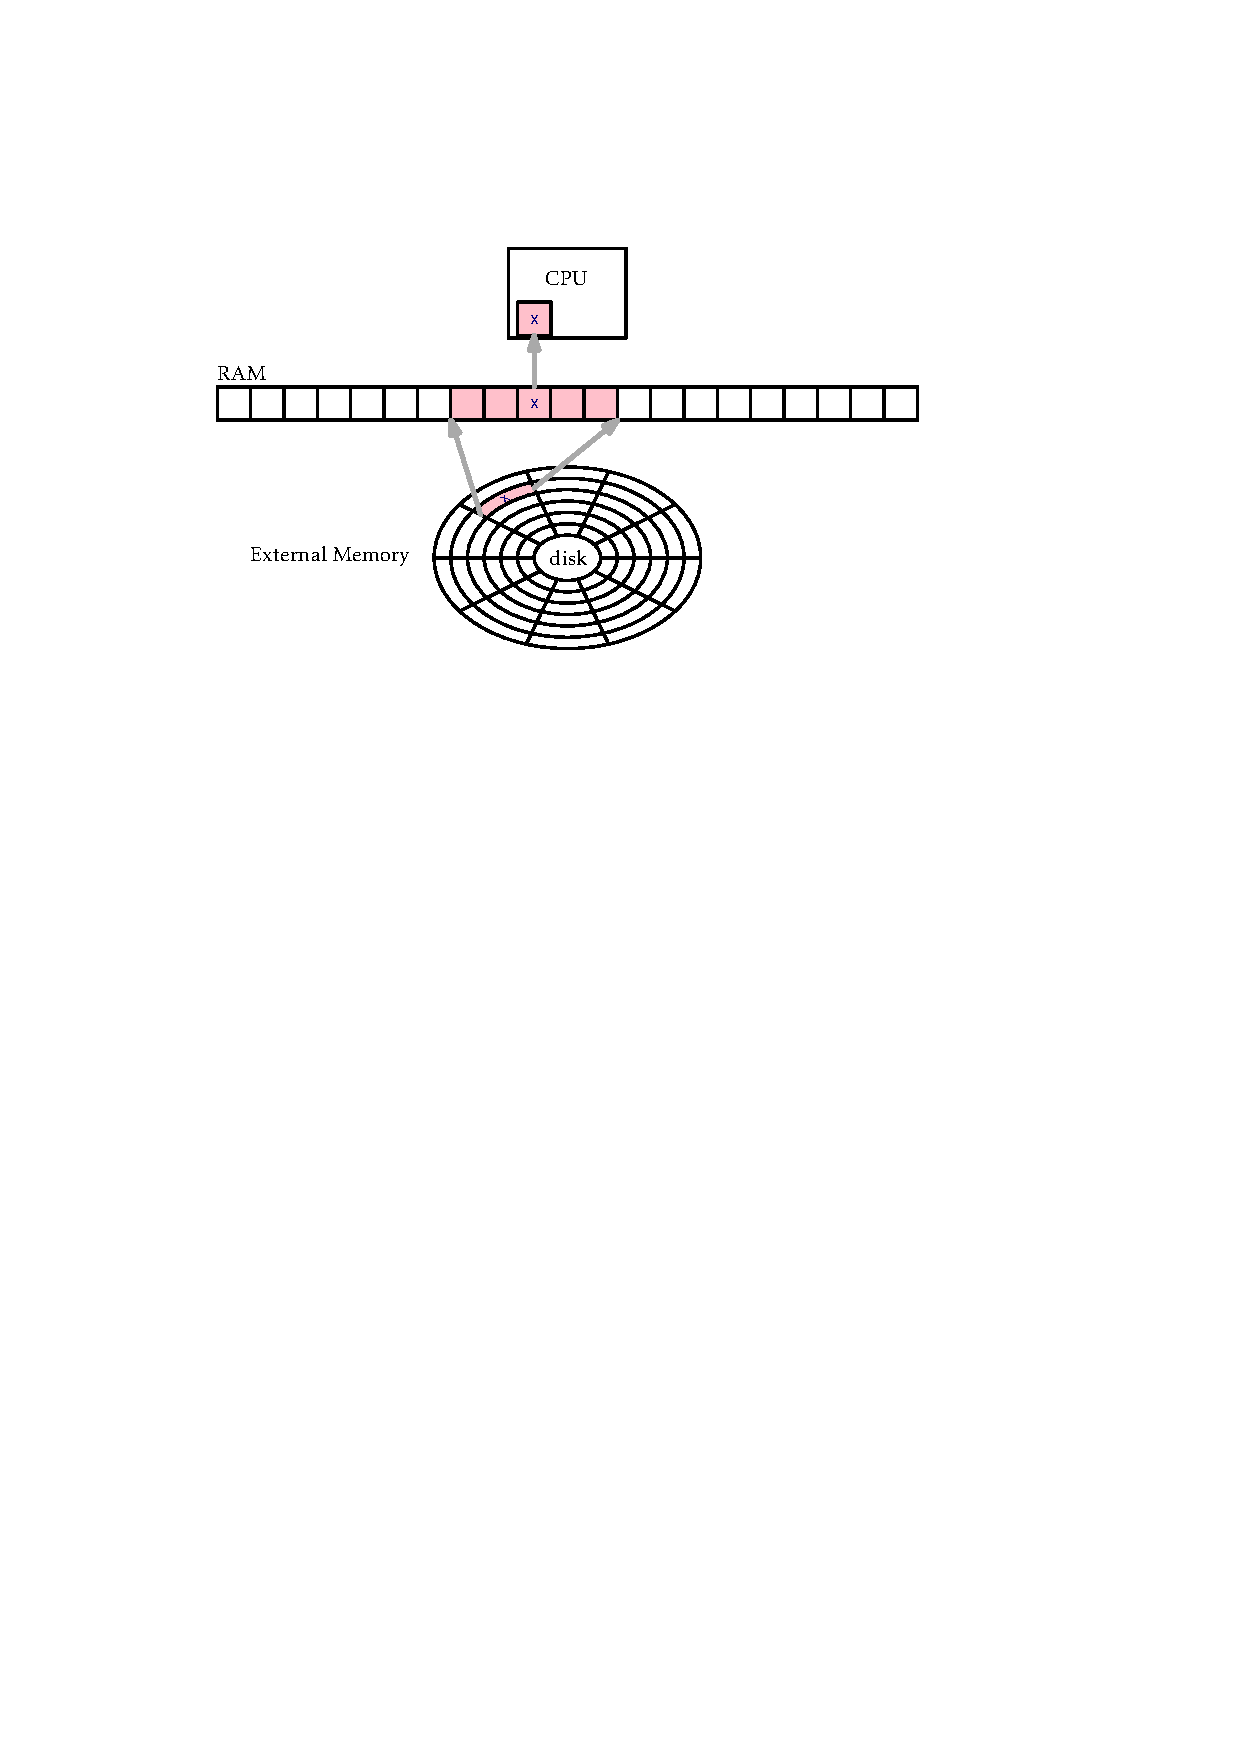
\includegraphics[width=\ScaleIfNeeded]{figs/em}}
  \caption[O modelo de memória externa]{No modelo de memória externa, acessar um item individual, #x#, na memória externa requer a leitura de todo o bloco contendo #x# na RAM.}
  \figlabel{em}
\end{figure}

No modelo de memória externa completo, o tamanho da memória interna também é um parâmetro. Porém, para as estruturas de dados descritas neste capítulo, é suficiente ter uma memória interna de tamanho $O(B+\log_B #n#)$. Ou seja, a memória precisa ser capaz de armazenar um número constante de blocos e uma pilha de recursão de altura $O(\log_B #n#)$. Na maioria dos casos, o termo $O(B)$ domina o requisito de memória.
Por exemplo, mesmo com o valor relativamente pequeno $B=32$, $B\ge \log_B #n#$ para todos $#n#\le 2^{160}$. Em decimal, $B\ge \log_B #n#$ para qualquer
\[
#n# \le 1\,461\,501\,637\,330\,902\,918\,203\,684\,832\,716\,283\,019\,655\,932\,542\,976 \enspace 
. \]

\section{O Armazém de Blocos - BlockStore}

\index{armazém de blocos}%
\index{BlockStore@#BlockStore#}%
A noção de memória externa inclui um grande número de dispositivos diferentes possíveis, cada um dos quais tem seu próprio tamanho de bloco e é
acessado com sua própria coleção de chamadas de sistema. Para simplificar a exposição deste capítulo para que possamos nos concentrar nas ideias comuns, encapsulamos dispositivos de memória externa com um objeto chamado #BlockStore#.
Um #BlockStore# armazena uma coleção de blocos de memória, cada um com o tamanho $B$.
Cada bloco é identificado exclusivamente por seu índice inteiro. Um #BlockStore# oferece suporte a estas operações:
\begin{enumerate}
  \item #readBlock(i)#: Retorna o conteúdo do bloco cujo índice é #i#.

  \item #writeBlock(i,b)#: Grave o conteúdo de #b# no bloco cujo índice é #i#.

  \item #placeBlock(b)#: Retorne um novo índice e armazene o conteúdo de #b# neste índice.

  \item #freeBlock(i)#: Libere o bloco cujo índice é #i#. Isso indica que o conteúdo deste bloco não é mais usado, então a memória externa alocada por este bloco pode ser reutilizada.
\end{enumerate}

A maneira mais fácil de imaginar um #BlockStore# é imaginá-lo armazenando um arquivo em disco que é particionado em blocos, cada um contendo $B$ bytes.
Desta forma, #readBlock(i)# e #writeBlock(i,b)# simplesmente lêem e gravam os bytes $#i#B,\ldots,(#i#+1)B-1$ deste arquivo. Além disso, um #BlockStore# simples pode manter uma \emph{lista livre} de blocos que estão disponíveis para uso. Os blocos liberados com #freeBlock(i)# são adicionados à lista livre.
Desta forma, #placeBlock(b)# pode usar um bloco da lista livre ou, se nenhum estiver disponível, acrescentar um novo bloco ao final do arquivo.


\section{Árvores B (B-Trees)}
\seclabel{btree}

Nesta seção, discutimos uma generalização de árvores binárias, chamadas de árvores $B$, que são eficientes no modelo de memória externa.
Alternativamente, árvores $B$ podem ser vistos como a generalização natural de árvores 2-4  descritas em \secref{twofour}. (Uma árvore 2-4 é um caso especial de árvore $B$ que obtemos definindo $B=2$.)

\index{arvore@árvore $B$@árvore $B$}%
\index{arvore B@árvore $B$}%
Para qualquer inteiro $B\ge 2$, uma \emph {árvore $B$} é uma árvore em que todas as folhas têm a mesma profundidade e cada nó interno não raiz, #u#, tem pelo menos $B$ filhos e no máximo $2B$ filhos. Os filhos de #u# são armazenados em uma matriz, #u.children#. O número necessário de filhos é relaxado na raiz, podendo ter entre 2 e $2B$ filhos.

Se a altura de uma árvore $B$ é $h$, segue-se que o número, $\ell$, de folhas na árvore $B$ satisfaz
\[
    2B^{h-1} \le \ell \le (2B)^{h} \enspace .
\]
Tomando o logaritmo da primeira desigualdade e reorganizando os termos, obtém-se:
\begin{align*}
    h & \le \frac{\log \ell-1}{\log B} + 1  \\
      & \le \frac{\log \ell}{\log B} + 1 \\
      & = \log_B \ell + 1 \enspace .
\end{align*}
Ou seja, a altura de uma árvore $B$ é proporcional ao logaritmo de base $B$ do número de folhas.

Cada nó, #u#, na árvore $B$ armazena uma matriz de chaves
$#u.keys#[0],\ldots,#u.keys#[2B-1]$. Se #u# for um nó interno com $k$ filhos, então o número de chaves armazenadas em #u# é exatamente $k-1$ e estas são armazenadas em $#u.keys#[0],\ldots,#u.keys#[k-2]$. As entradas restantes da matriz $2B-k+1$ em #u.keys# são definidas como #null#. Se #u# for um nó folha não raiz, então #u# contém entre as chaves $B-1$ e $2B-1$. As chaves em uma árvore $B$ respeitam uma ordem semelhante às chaves em uma árvore de pesquisa binária.
Para qualquer nó, #u#, que armazena $k-1$ chaves,
\[
   #u.keys[0]# < #u.keys[1]# < \cdots < #u.keys#[k-2] \enspace .
\]
Se #u# for um nó interno, então para cada $#i#\in\{0,\ldots,k-2\}$,
$#u.keys[i]#$ é maior do que todas as chaves armazenadas na subárvore com raiz em #u.children[i]#, mas menor do que todas as chaves armazenadas na subárvore com raiz em $#u.children[i+1]#$.  Informalmente,
\[
   #u.children[i]# \prec #u.keys[i]# \prec #u.children[i+1]# \enspace .
\]
Um exemplo de uma árvore $B$ com $B=2$ é mostrado na \figref{btree}.

\begin{figure}
  \centering{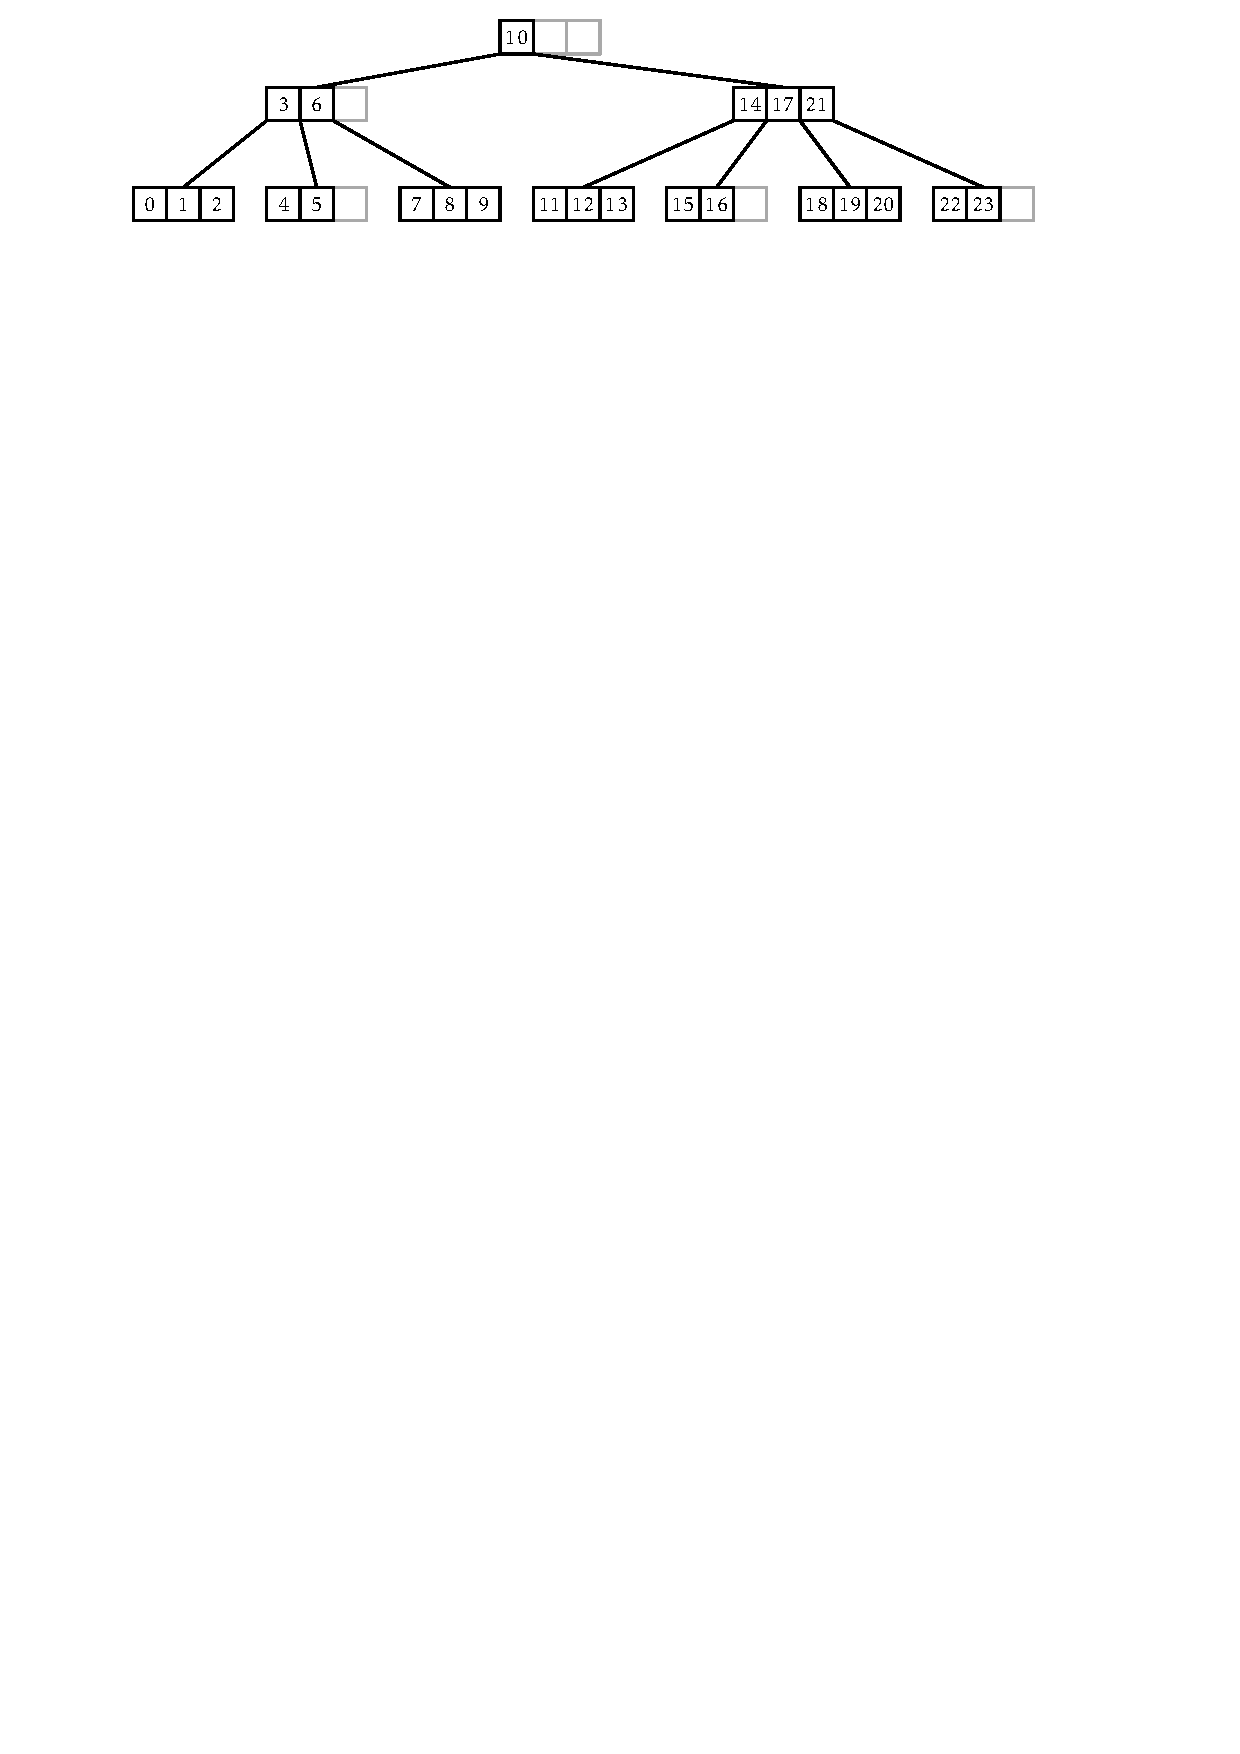
\includegraphics[width=\ScaleIfNeeded]{figs/btree-1}}
  \caption{Uma árvore $B$ com $B=2$.}
  \figlabel{btree}
\end{figure}

Observe que os dados armazenados em um nó da árvore $B$ têm o tamanho $O(B)$. Portanto, em uma configuração de memória externa, o valor de $B$ em uma árvore $B$ é escolhido de forma que um nó caiba em um único bloco de memória externa. Desta forma, o tempo que leva para realizar uma operação na árvore $B$ no modelo de memória externa é proporcional ao número de nós que são acessados (lidos ou gravados) pela operação.

Por exemplo, se as chaves são inteiros de 4 bytes e os índices dos nós também são 4 bytes, então definir $B=256$ significa que cada nó armazena
\[
(4+4)\times 2B
 = 8\times512=4096
\]
bytes de dados. Este seria um valor perfeito de $B$ para o disco rígido ou unidade de estado sólido discutida na introdução deste capítulo, que tem um tamanho de bloco de $4096$ bytes.

A classe #BTree#, que implementa uma árvore $B$, armazena um #BlockStore#, #bs#, que armazena #BTree# nós, bem como o índice, #ri#, do nó raiz. Como de costume, um número inteiro, #n#, é usado para controlar o número de itens na estrutura de dados:
\cppimport{ods/BTree.n.ri.bs}
\javaimport{ods/BTree.n.ri.bs}
\pcodeimport{ods/BTree.initialize(b)}

\subsection{Busca}

A implementação da operação #find(x)#, ilustrada em \figref{btree-find}, generaliza a operação #find(x)# em uma árvore de pesquisa binária. A pesquisa por #x# começa na raiz e usa as chaves armazenadas em um nó, #u#, para determinar em qual dos filhos de #u# a pesquisa deve continuar.

\begin{figure}
  \centering{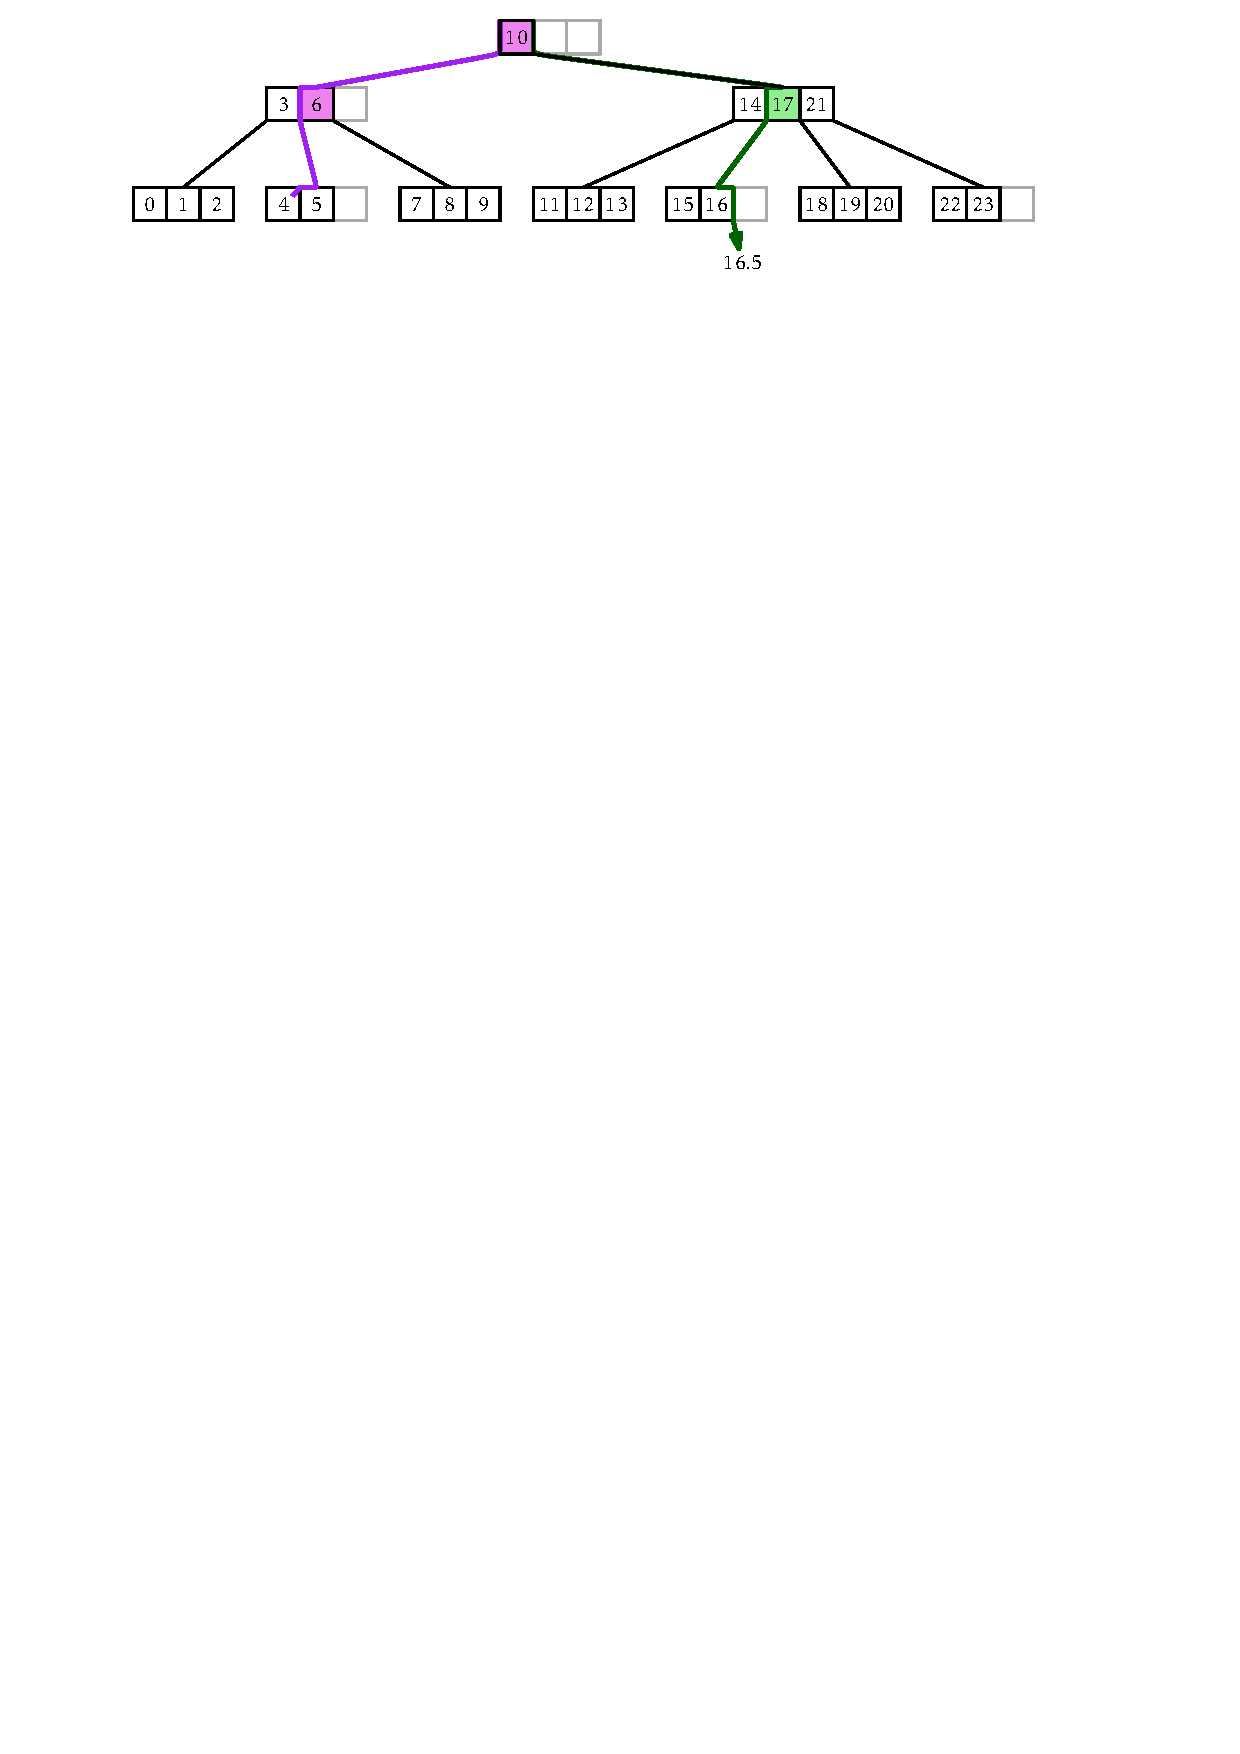
\includegraphics[width=\ScaleIfNeeded]{figs/btree-2}}
  \caption[Pesquisando em uma árvore $B$]{Uma pesquisa bem-sucedida (pelo valor 4) e uma pesquisa malsucedida (pelo valor 16.5) em uma árvore $B$. Os nós sombreados mostram onde o valor de #z# é atualizado durante as pesquisas.}
  \figlabel{btree-find}
\end{figure}
Mais especificamente, em um nó #u#, a pesquisa verifica se #x# está armazenado em #u.keys#. Nesse caso, #x# foi encontrado e a pesquisa foi concluída.
Caso contrário, a pesquisa encontra o menor inteiro, #i#, de modo que $#u.keys[i]#>#x#$ e continua a pesquisa na subárvore com raiz em #u.children[i]#. Se nenhuma chave em #u.keys# for maior que #x#, a busca continua no filho mais à direita de #u#. Assim como as árvores de busca binária, o algoritmo rastreia a chave vista mais recentemente, #z#, que é maior do que #x#. Caso #x# não seja encontrado, #z# é retornado como o menor valor maior ou igual a #x#.
\codeimport{ods/BTree.find(x)}
Central para o método #find(x)# é o método #findIt(a,x)# que pesquisa em um array ordenado completado com  #null#, #a#, pelo valor #x#.
Este método, ilustrado em \figref{findit}, funciona para qualquer array, #a#, onde $#a#[0],\ldots,#a#[k-1]$ é uma sequência de chaves em ordem classificada e $#a#[k],\ldots,#a#[#a.length#-1]$ estão todos configurados para #null#.
Se #x# estiver na matriz na posição #i#, então #findIt(a, x)# retorna $-#i#-1$. Caso contrário, ele retorna o menor índice, #i#, de modo que
$#a[i]#>#x#$ ou $#a[i]#=#null#$.
\begin{figure}
  \centering{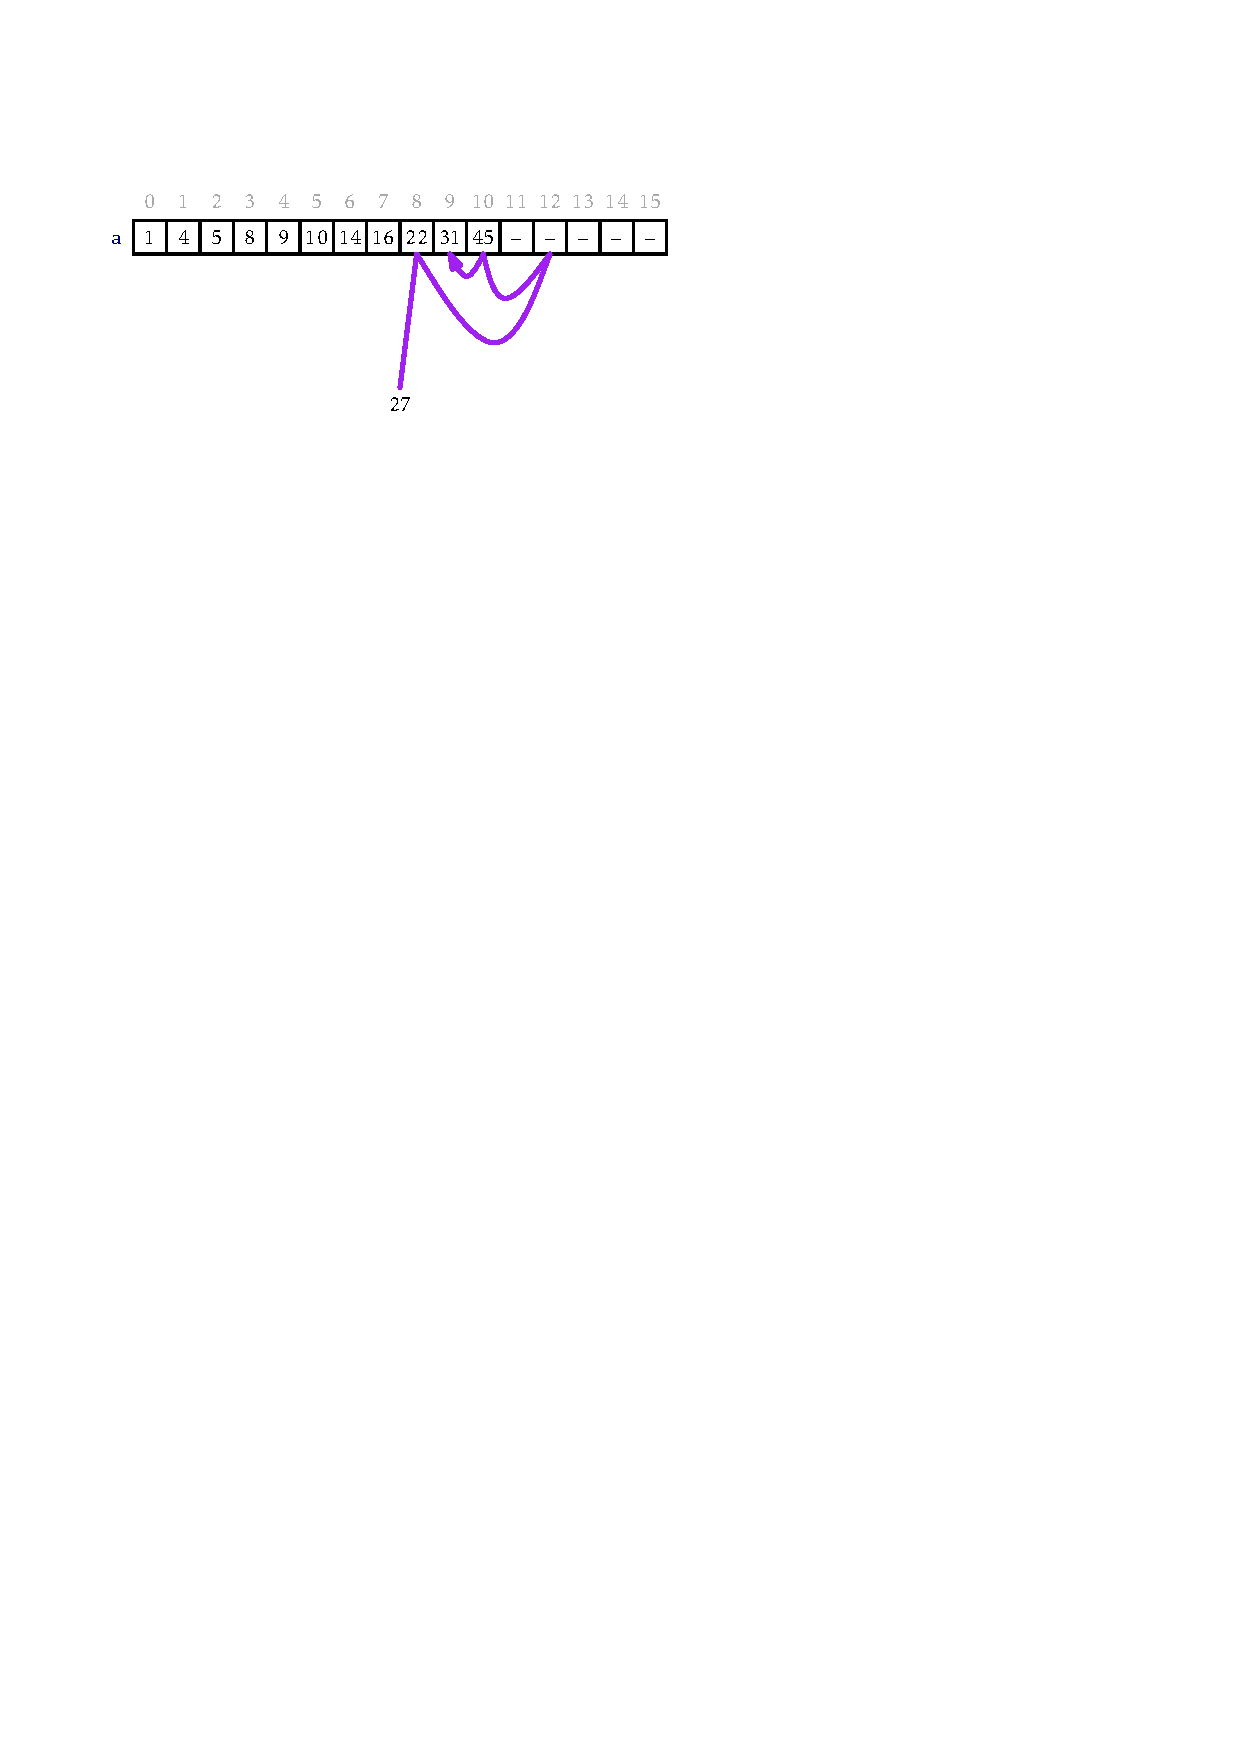
\includegraphics[scale=0.90909]{figs/findit}}
  \caption[O método findIt(a,x)]{A execução de #findIt(a,27)#.}
  \figlabel{findit}
\end{figure}
\codeimport{ods/BTree.findIt(a,x)}
O método #findIt(a,x)# usa uma pesquisa binária
\index{pesquisa binária}%
que divide pela metade o espaço de pesquisa em cada etapa, para que seja executado em um tempo $O(\log(#a.length#))$.  Em nosso ambiente, $#a.length#=2B$, assim #findIt(a,x)# executa em tempo $O(\log B)$.

Podemos analisar o tempo de execução de uma operação #find(x)# em uma árvore $B$,  tanto no modelo de palavra-RAM usual (onde cada instrução conta) quanto no modelo de memória externa (onde contamos apenas o número de nós acessados).
Uma vez que cada folha em uma árvore $B$ armazena pelo menos uma chave e a altura de uma árvore $B$ com $\ell$ folhas é $O(\log_B\ell)$, a altura de uma árvore $B$ que armazena #n# chaves é $O(\log_B#n#)$. Portanto, no modelo de memória externa, o tempo gasto pela operação #find(x)# é $O(\log_B#n#)$. Para determinar o tempo de execução no modelo palavra-RAM, temos que contabilizar o custo de chamar #findIt(a,x) # para cada nó que acessamos, portanto, o tempo de execução de #find(x)# no modelo de palavra-RAM é
\[
   O(\log_B #n#)\times O(\log B) = O(\log #n#) \enspace .
\]

\subsection{Adição}

Uma diferença importante entre as árvores $B$ e a estrutura de dados #BinarySearchTree# de \secref{binarysearchtree} é que os nós de uma árvore $B$ não armazenam ponteiros para seus pais. A razão para isso será explicada em breve. A falta de ponteiros pai significa que as operações #add(x)# e #remove(x)# nas árvores $B$ são mais facilmente implementadas usando recursão.

Como todas as árvores de pesquisa balanceadas, alguma forma de rebalanceamento é necessária durante uma operação #add(x)#. Em uma árvore $B$, isso é feito por \emph{divisão} de nós.
\index{divisão}%
Referir-se à \figref{btree-split} para o que segue.
Embora a divisão ocorra em dois níveis de recursão, ela é melhor entendida como uma operação que pega um nó #u# contendo $2B$ chaves e tendo $2B+1$ filhos. Ele cria um novo nó, #w#, que adota $#u.children#[B],\ldots,#u.children#[2B]$. O novo nó #w# também pega as chaves maiores $B$ de #u#, $#u.keys# B],\ldots,#u.keys#[2B-1]$.
Neste ponto, #u# tem $B$ filhos e $B$ chaves. A chave extra, $#u.keys#[B-1]$, é passada para o pai de #u#, que também adota #w#.

Observe que a operação de divisão modifica três nós: #u#, #u# pai e o novo nó, #w#. É por isso que é importante que os nós de uma árvore $B$ não mantenham ponteiros para os pais. Se o fizessem, então os $B+1$ filhos adotados por #w# precisariam ter seus ponteiros para os pais modificados. Isso aumentaria o número de acessos à memória externa de 3 para $B+4$ e tornaria as árvores $B$ muito menos eficientes para grandes valores de $B$.

\begin{figure}
   \centering{\begin{tabular}{@{}l@{}}
     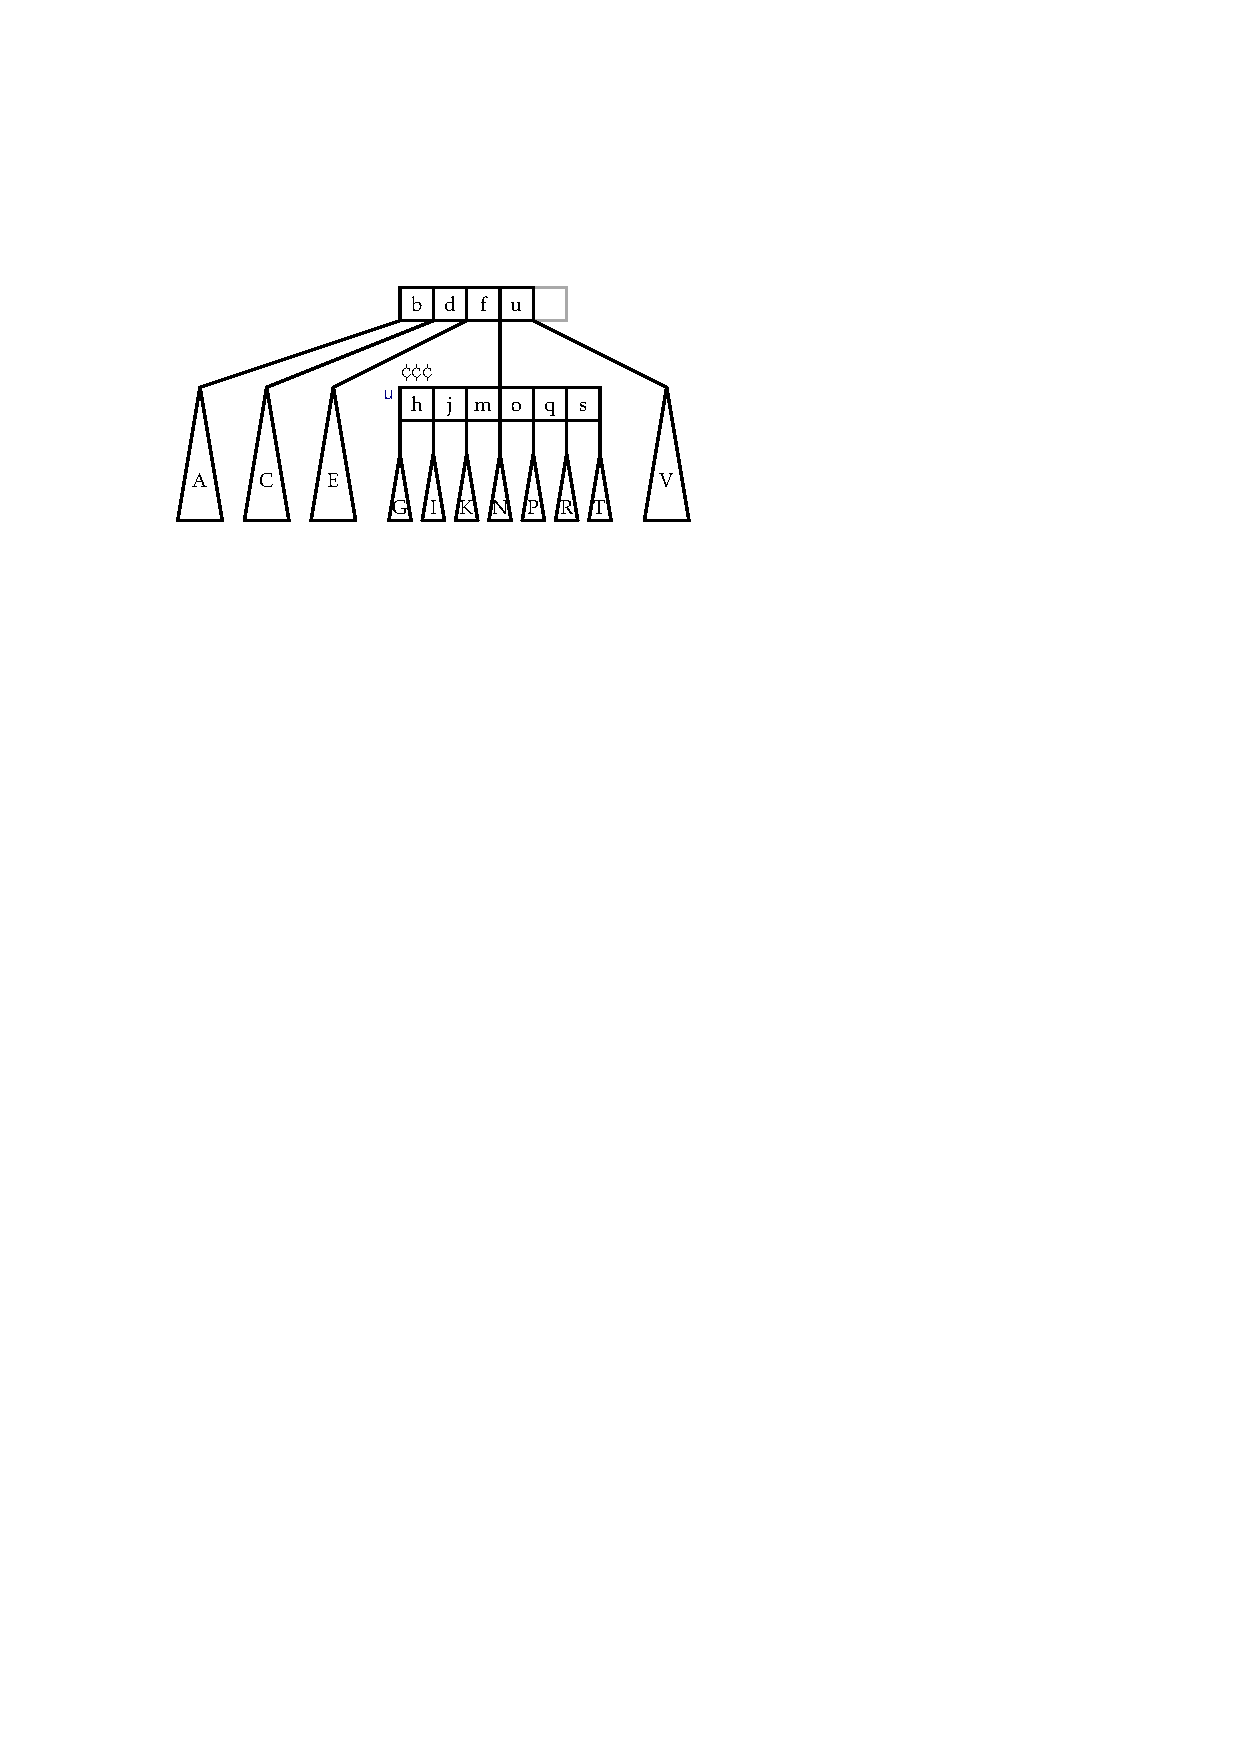
\includegraphics[width=\ScaleIfNeeded]{figs/btree-split-1} \\[2ex]
     \multicolumn{1}{c}{#u.split()#} \\ 
     \multicolumn{1}{c}{$\Downarrow$} \\[2ex]
     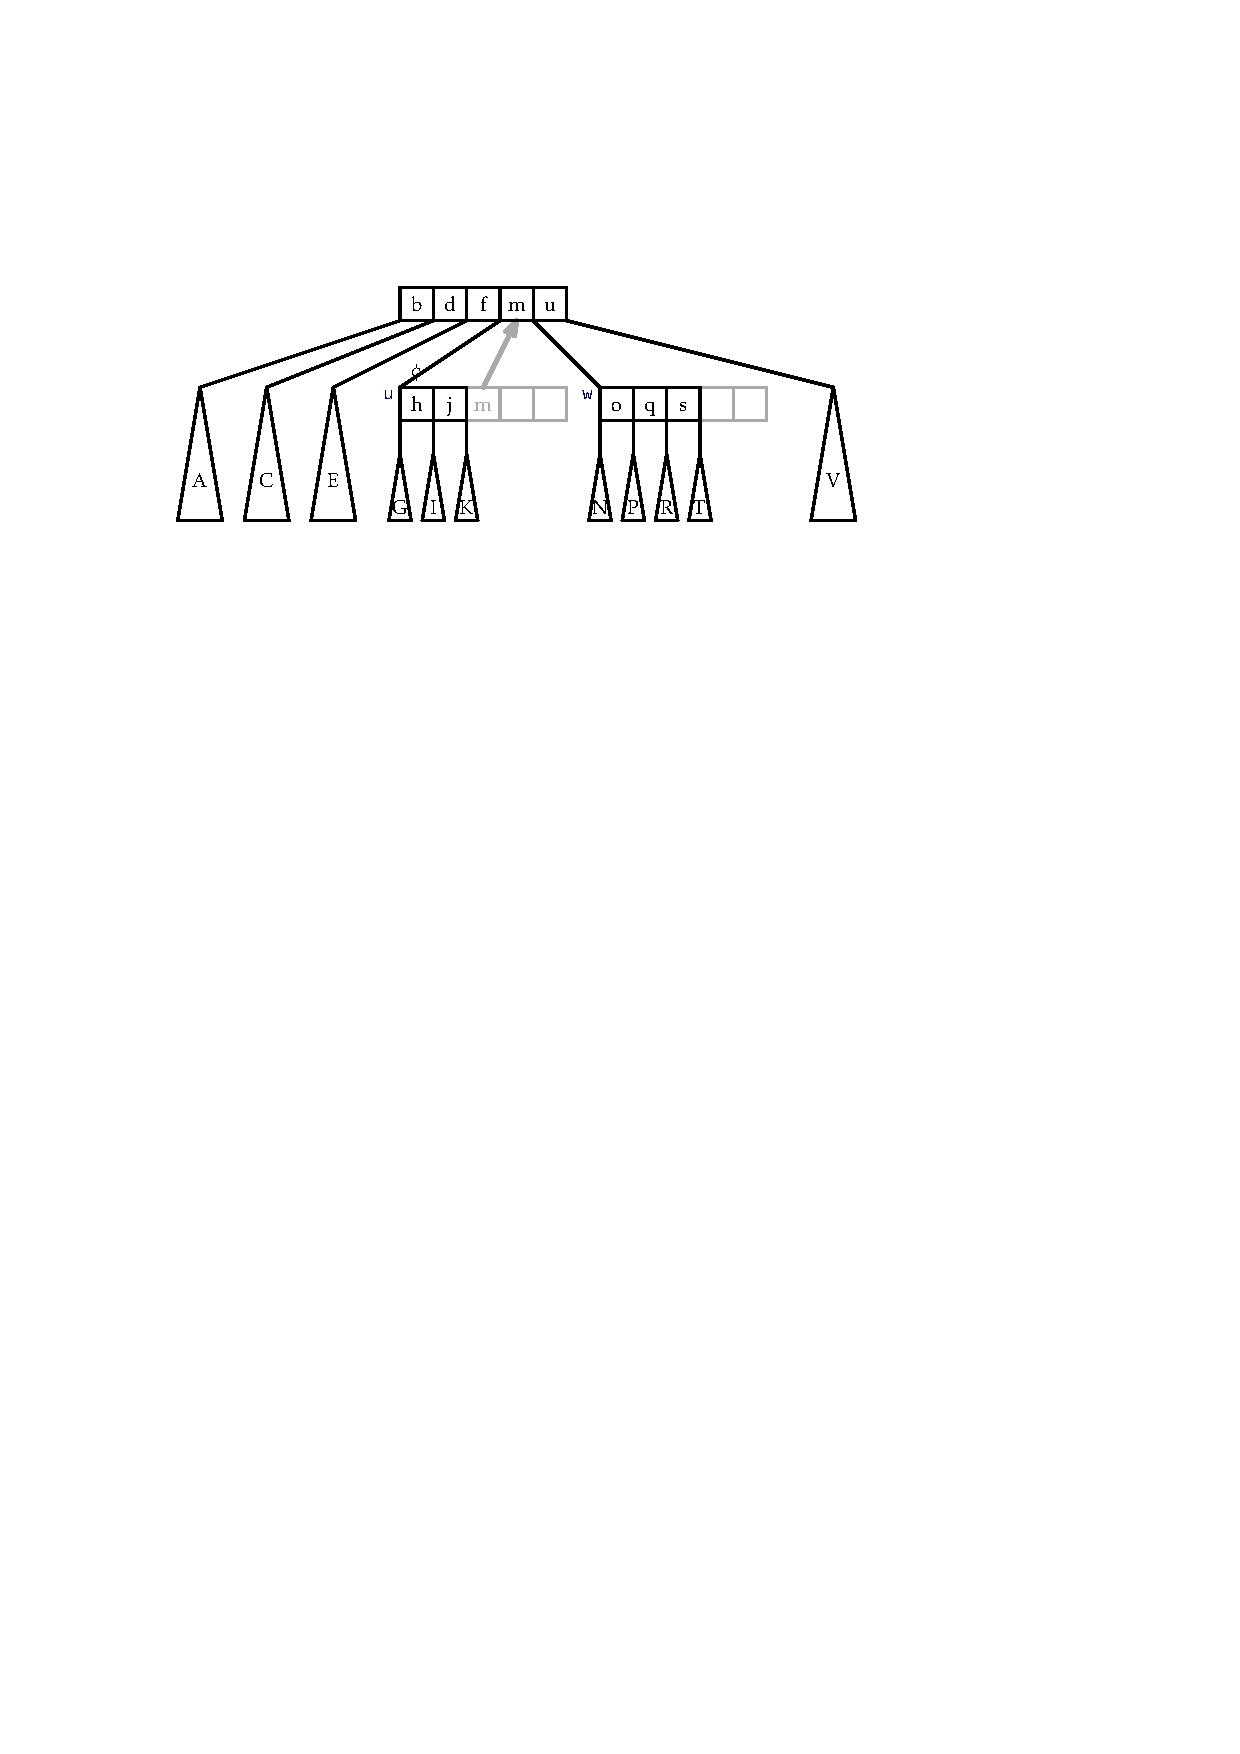
\includegraphics[width=\ScaleIfNeeded]{figs/btree-split-2} \\
   \end{tabular}}
   \caption[Dividindo um nó de árvore $B$]{Dividindo o nó #u# em uma
     árvore $B$ ($B=3$). Observe que a chave $#u.keys#[2]=\mathrm{m}$
     passa de #u# para seu pai.}
   \figlabel{btree-split}
\end{figure}

O método #add(x)# em uma árvore $B$ é ilustrado em \figref{btree-add}.
Em um nível superior, este método encontra uma folha, #u#, na qual adicionar o valor #x#. Se isso fizer com que #u# fique cheio demais (porque já continha $B-1$ chaves), então #u# será dividido. Se isso fizer com que o pai de #u# fique cheio demais, então o pai de #u# também é dividido, o que pode fazer com que o avô de #u# fique cheio demais, e assim por diante. Este processo continua, subindo na árvore um nível de cada vez até chegar a um nó que não está lotado ou até que a raiz seja dividida. No primeiro caso, o processo para. No último caso, uma nova raiz é criada cujos dois filhos se tornam os nós obtidos quando a raiz original foi dividida.

\begin{figure}
   \centering{\begin{tabular}{@{}l@{}}
     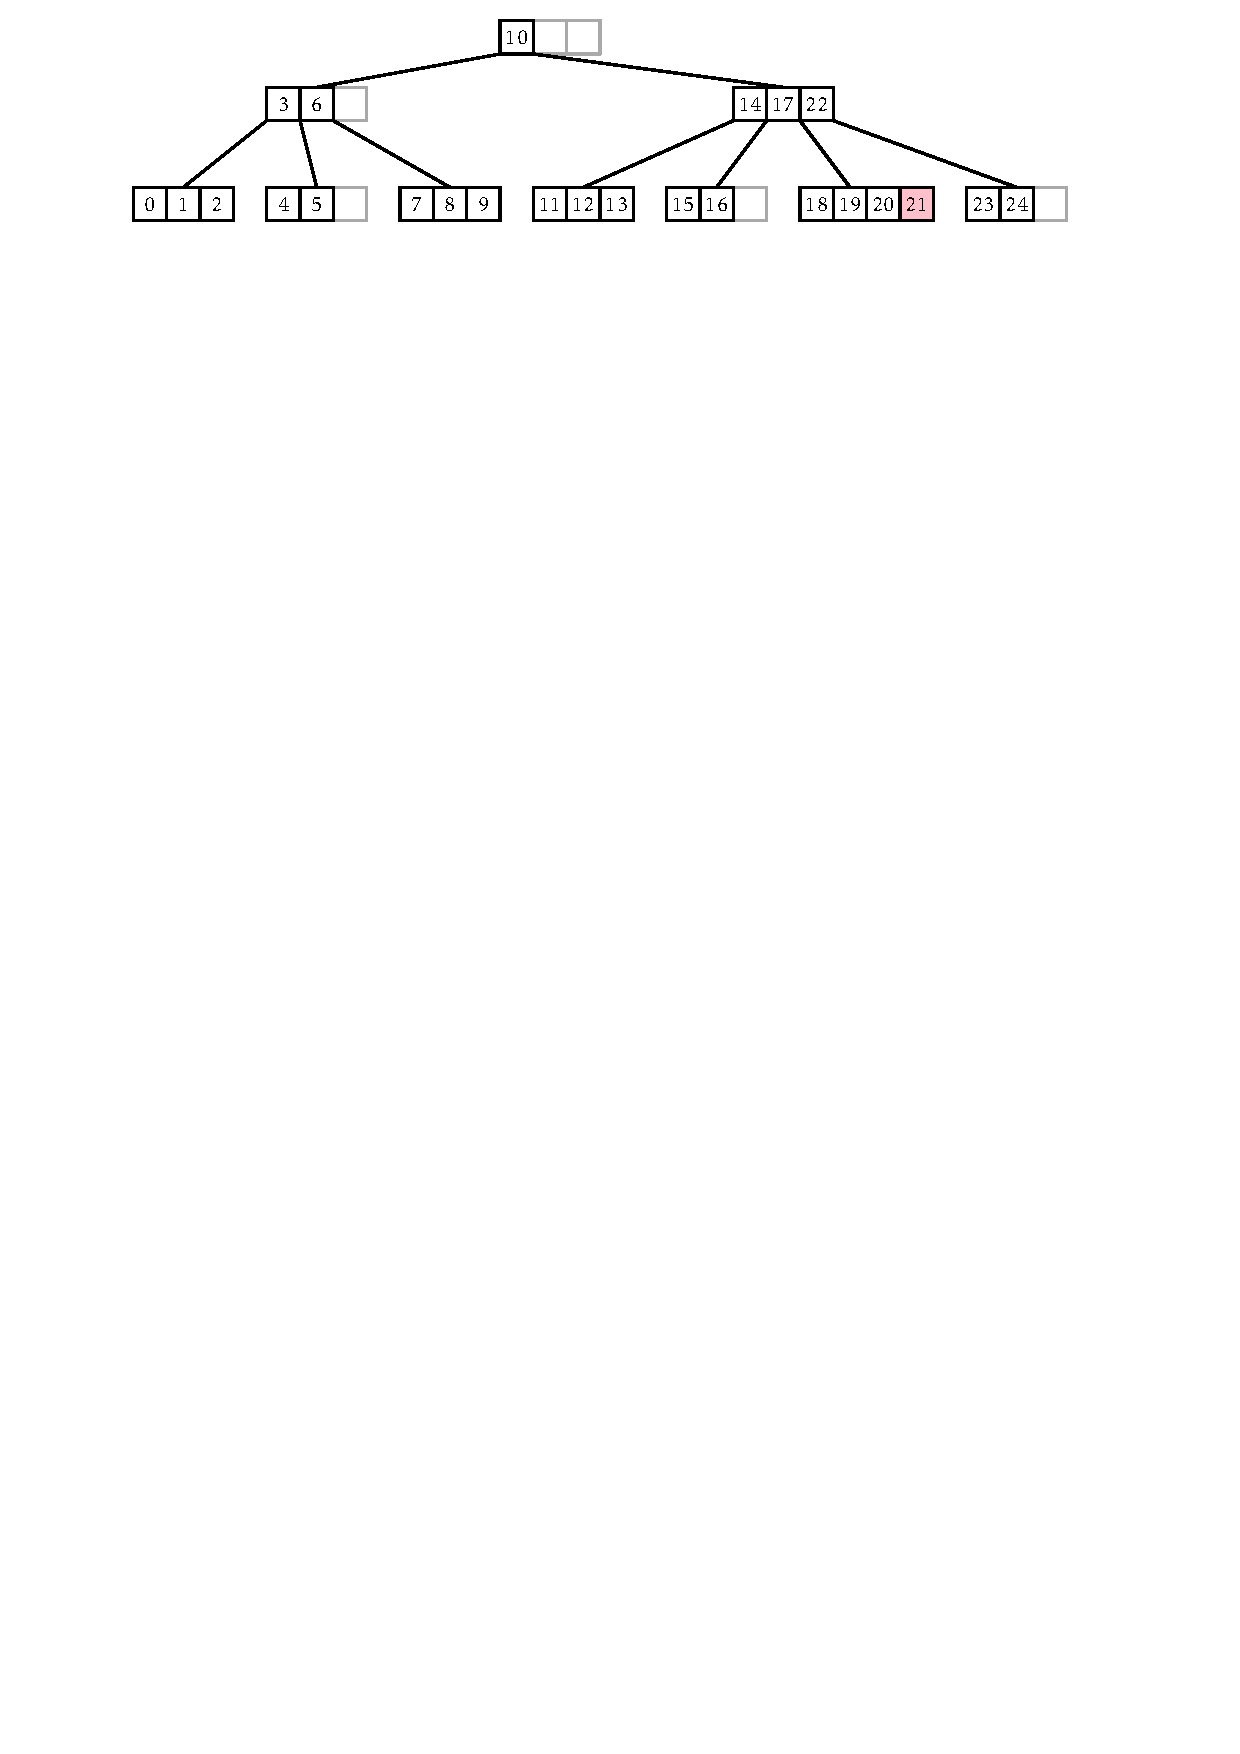
\includegraphics[width=\ScaleIfNeeded]{figs/btree-add-1} \\[2ex]
     \multicolumn{1}{c}{$\Downarrow$} \\[2ex]
     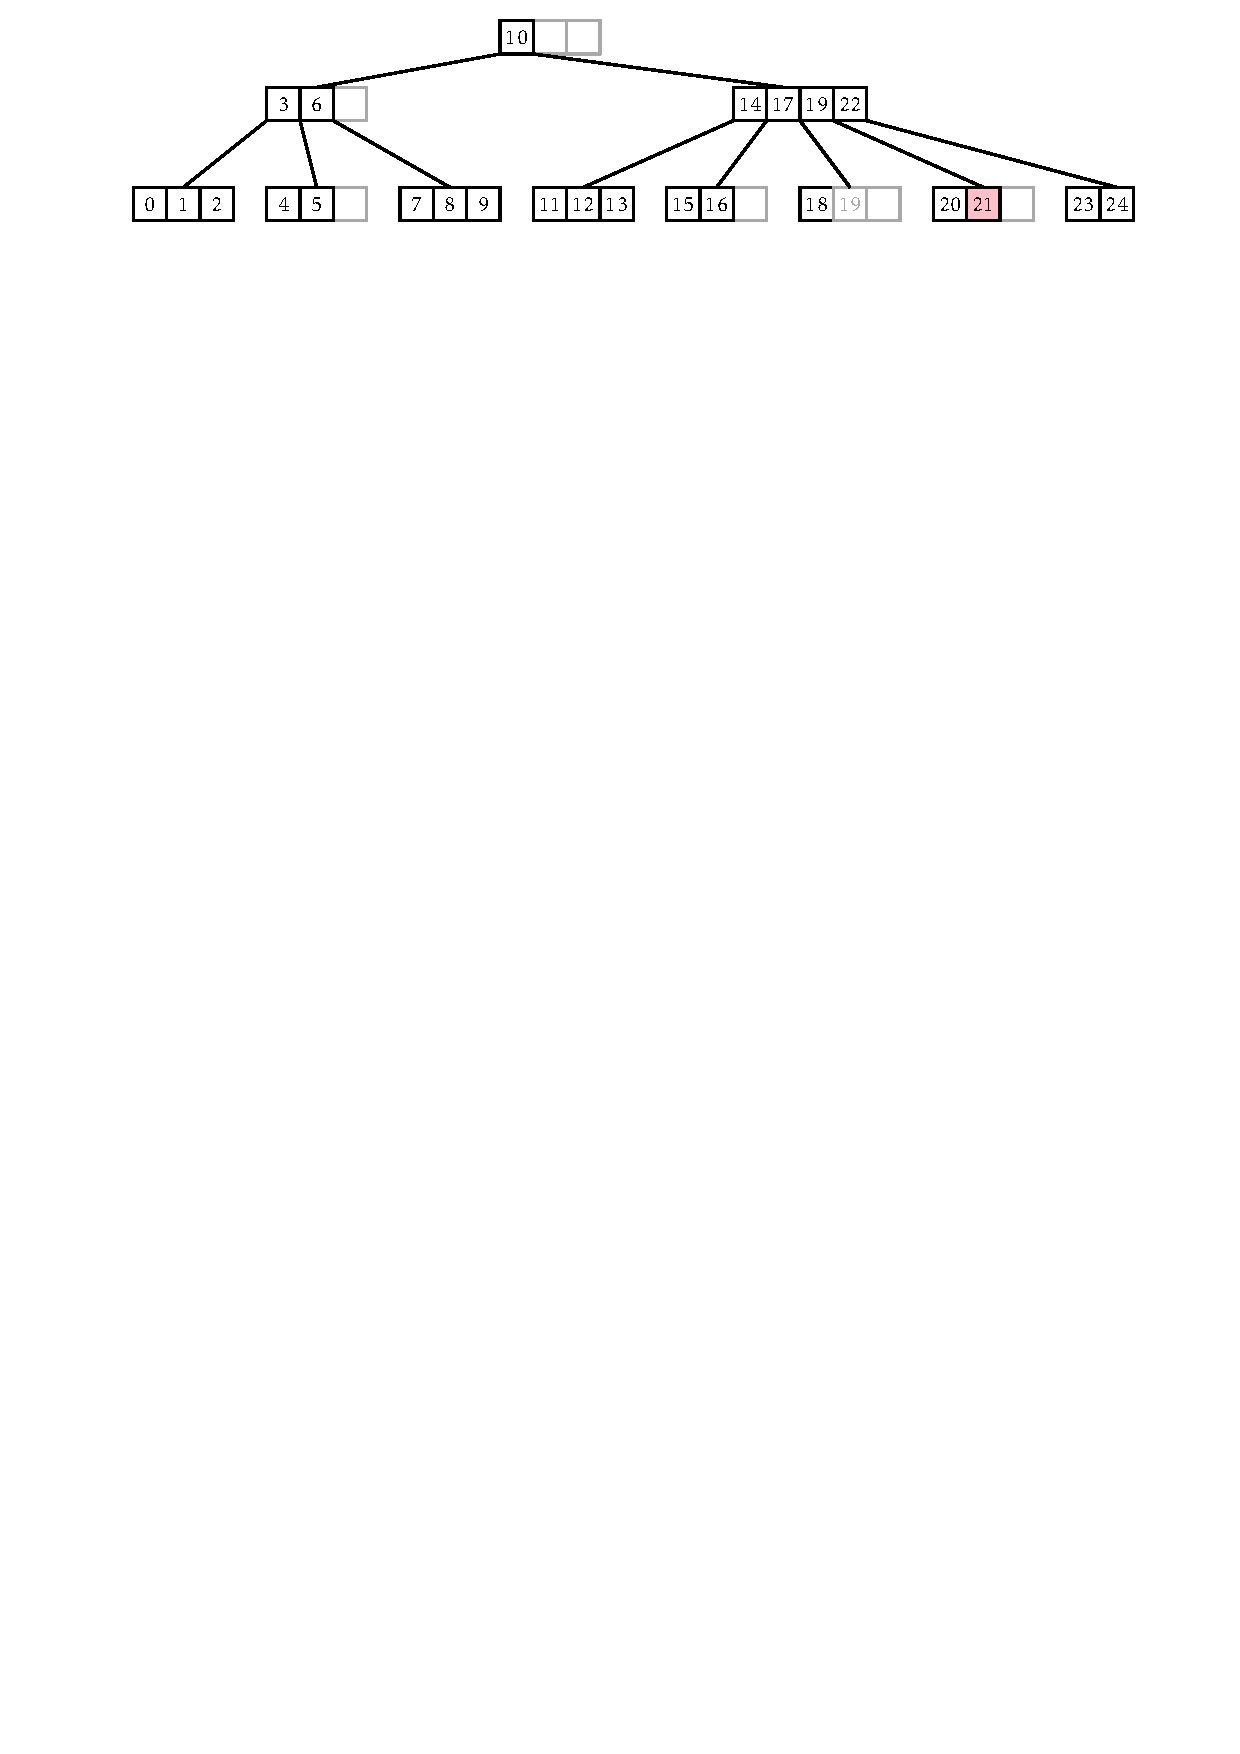
\includegraphics[width=\ScaleIfNeeded]{figs/btree-add-2} \\[2ex]
     \multicolumn{1}{c}{$\Downarrow$} \\[2ex]
     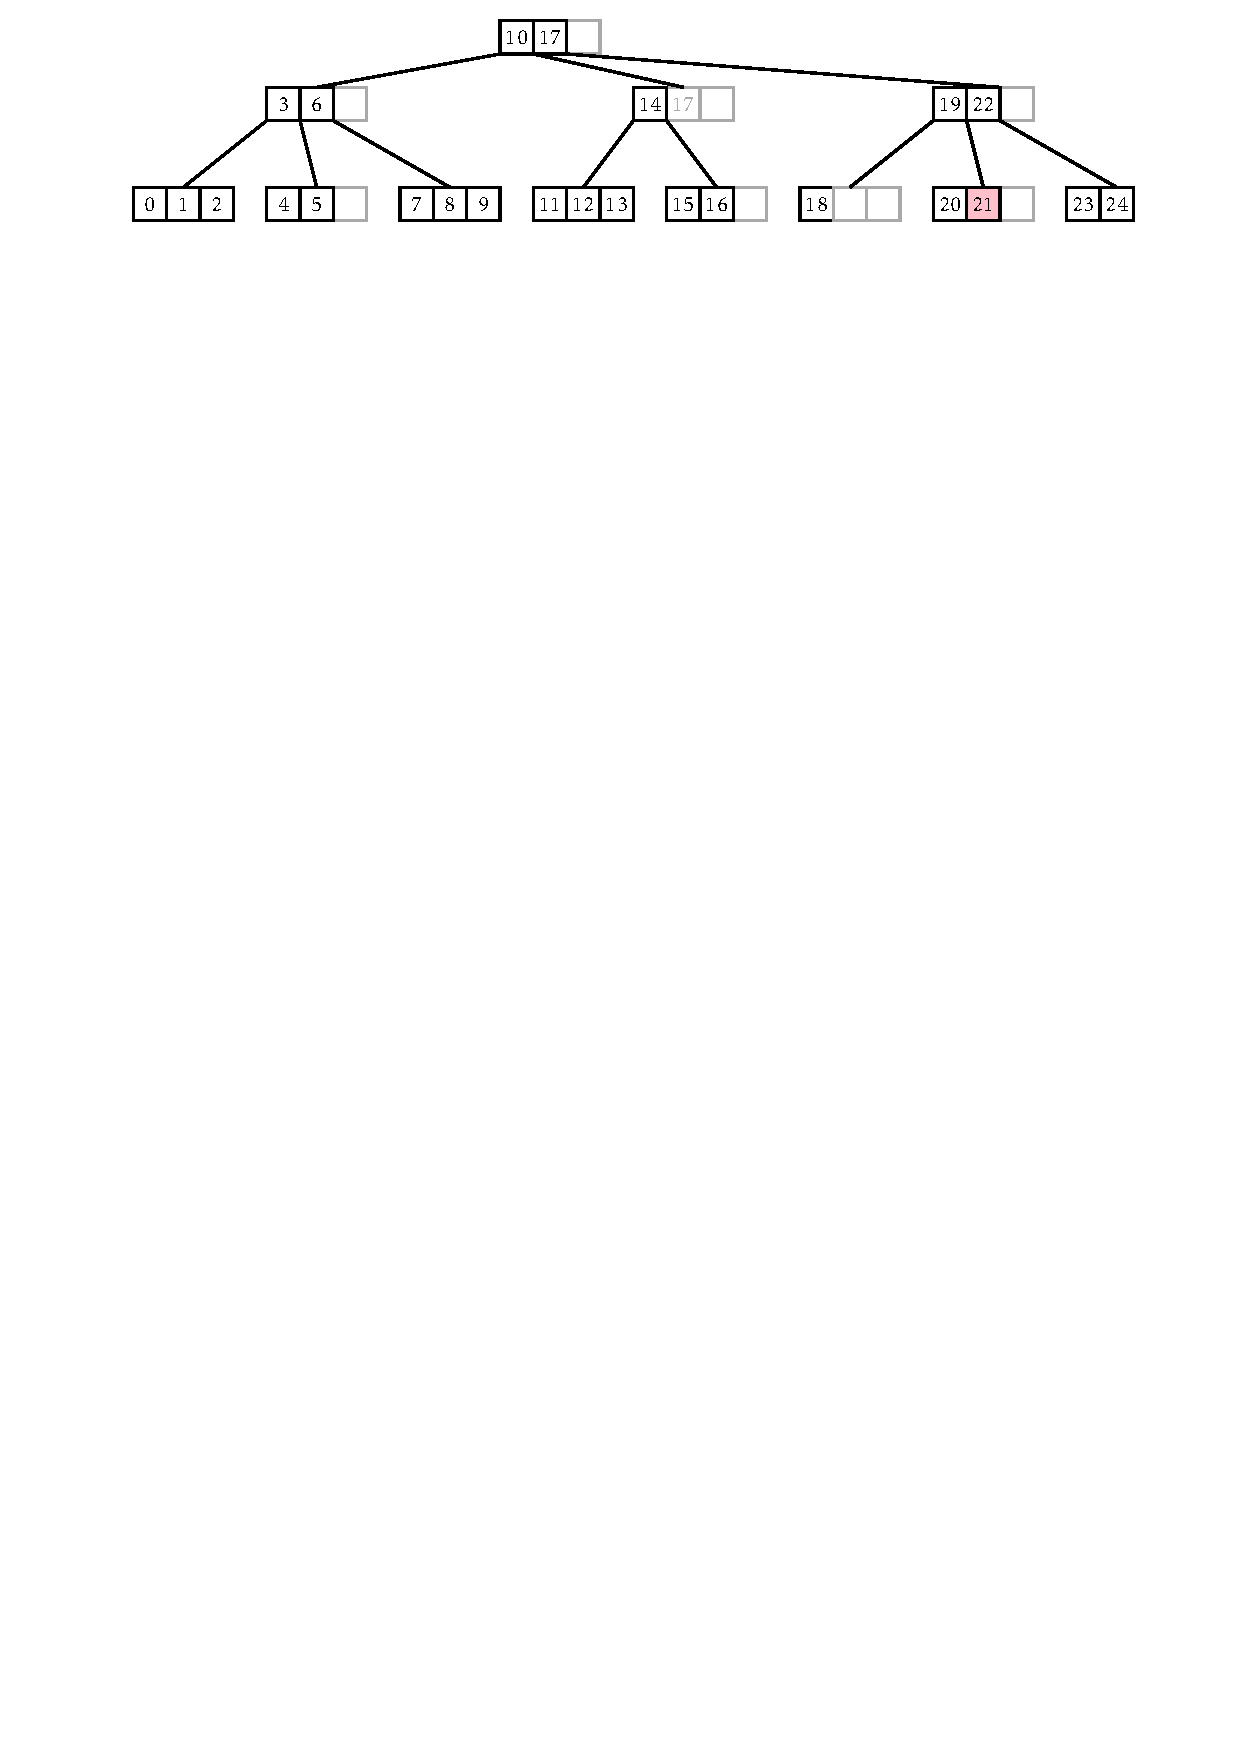
\includegraphics[width=\ScaleIfNeeded]{figs/btree-add-3} 
   \end{tabular}}
   \caption[Adicionando a uma árvore $B$]{A operação #add(x)# em uma #BTree#. Adicionar o valor 21 resulta na divisão de dois nós.}
   \figlabel{btree-add}
\end{figure}

O resumo da execução do método #add(x)# é que ele caminha da raiz para uma folha em busca de #x#, adiciona #x# a esta folha e, em seguida, sobe de volta para a raiz, dividindo quaisquer nós excessivamente cheios que encontrar ao longo do caminho. Com essa visão de alto nível em mente, agora podemos nos aprofundar nos detalhes de como esse método pode ser implementado recursivamente.

O verdadeiro trabalho de #add(x)# é feito pelo método #addRecursive(x,ui)#, que adiciona o valor #x# à subárvore cuja raiz, #u#, tem o identificador #ui#. Se #u# for uma folha, então #x# é simplesmente inserido em #u.keys#. Caso contrário, #x# é adicionado recursivamente no filho apropriado, $#u#'$, de #u#. O resultado dessa chamada recursiva é normalmente #null#, mas também pode ser uma referência a um nó recém-criado, #w#, que foi criado porque $#u#'$ foi dividido. Neste caso, #u# adota #w# e pega sua primeira chave, completando a operação de divisão em $#u#'$.

Após o valor #x# ter sido adicionado (para #u# ou para um descendente de #u#), o método #addRecursive(x,ui)# verifica se #u# está armazenando muitas (mais de $2B-1$) chaves. Se sim, então #u# precisa ser \emph{dividido} com uma chamada para o método #u.split()#. O resultado de chamar #u.split()# é um novo nó que é usado como o valor de retorno para #addRecursive(x,ui)#.
\codeimport{ods/BTree.addRecursive(x,ui)}

O método #addRecursive(x,ui)# é um auxiliar para o método #add(x)#, que chama #addRecursive(x,ri)# para inserir #x# na raiz da árvore $B$.
Se #addRecursive(x,ri)# faz com que a raiz se divida, então uma nova raiz é criada e recebe como seus filhos a raiz antiga e o novo nó criado pela divisão da raiz antiga.
\codeimport{ods/BTree.add(x)}

O método #add(x)# e seu auxiliar, #addRecursive(x,ui)#, podem ser analisados em duas fases:

\begin{description}
  \item[Fase descendente:]
    Durante a fase descendente da recursão, antes de #x# ser adicionado, eles acessam uma sequência de #BTree# nós e chamam #findIt(a,x)# em cada nó.
    Tal como acontece com o método #find(x)#, isso leva um tempo $O(\log_B #n#)$ no modelo de memória externa e um tempo $O(\log #n#)$ no modelo palavra-RAM.
  
  \item[Fase ascendente:]
    Durante a fase ascendente da recursão, após a adição de #x#, esses métodos executam uma sequência de no máximo $O(\log_B #n#)$ divisões.
    Cada divisão envolve apenas três nós, portanto, esta fase leva um tempo$O(\log_B #n#)$  no modelo de memória externa. No entanto, cada divisão envolve mover $B$ chaves e filhos de um nó para outro, portanto, no modelo de palavra-RAM, isso leva um tempo $O(B\log #n#)$.
\end{description}

Lembre-se de que o valor de $B$ pode ser muito grande, muito maior do que $\log #n#$. Portanto, no modelo de palavra-RAM, adicionar um valor a uma árvore $B$ pode ser muito mais lento do que adicionar em uma árvore de pesquisa binária balanceada. Posteriormente, em \secref{btree-amortized}, mostraremos que a situação não é tão ruim; o número amortizado de operações de divisão feitas durante uma operação #add(x)# é constante. Isso mostra que o tempo de execução (amortizado) da operação #add(x)# no modelo palavra-RAM é $O(B+\log #n#)$.


\subsection{Remoção}

A operação #remove(x)# em uma #BTree# é, novamente, mais facilmente implementada como um método recursivo. Embora a implementação recursiva de #remove(x)# espalhe a complexidade por vários métodos, o processo geral, que é ilustrado em \figref{btree-remove-full}, é bastante direto. Ao embaralhar as chaves, a remoção é reduzida ao problema de remover um valor, $#x#'$, de alguma folha, #u#. Remover $#x#'$ pode deixar #u# com menos de $B-1$ chaves; esta situação é chamada de \emph{underflow}.
\index{underflow}%

\begin{figure}
   \centering{\begin{tabular}{@{}l@{}}
     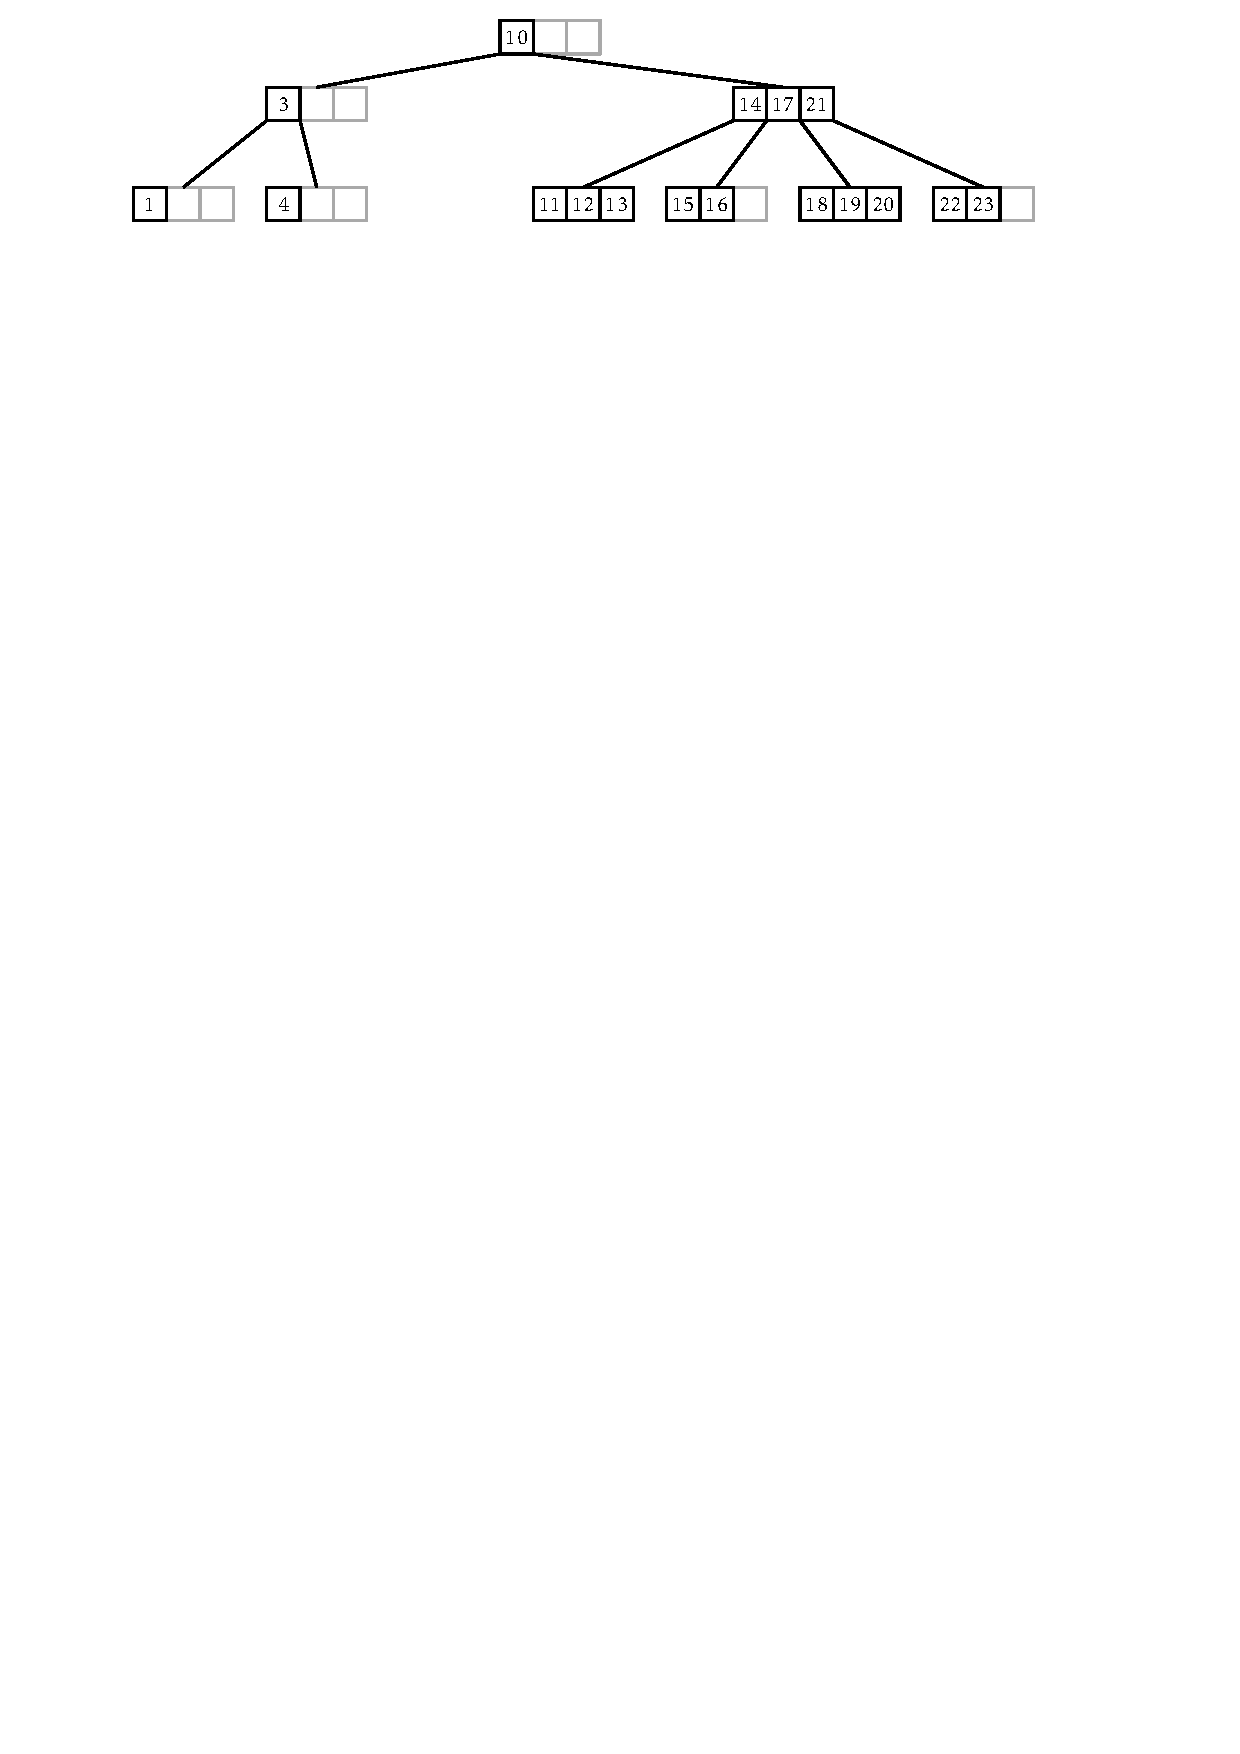
\includegraphics[width=\ScaleIfNeeded]{figs/btree-remove-full-1} \\[2ex]
     \multicolumn{1}{c}{$\Downarrow$} \\[2ex]
     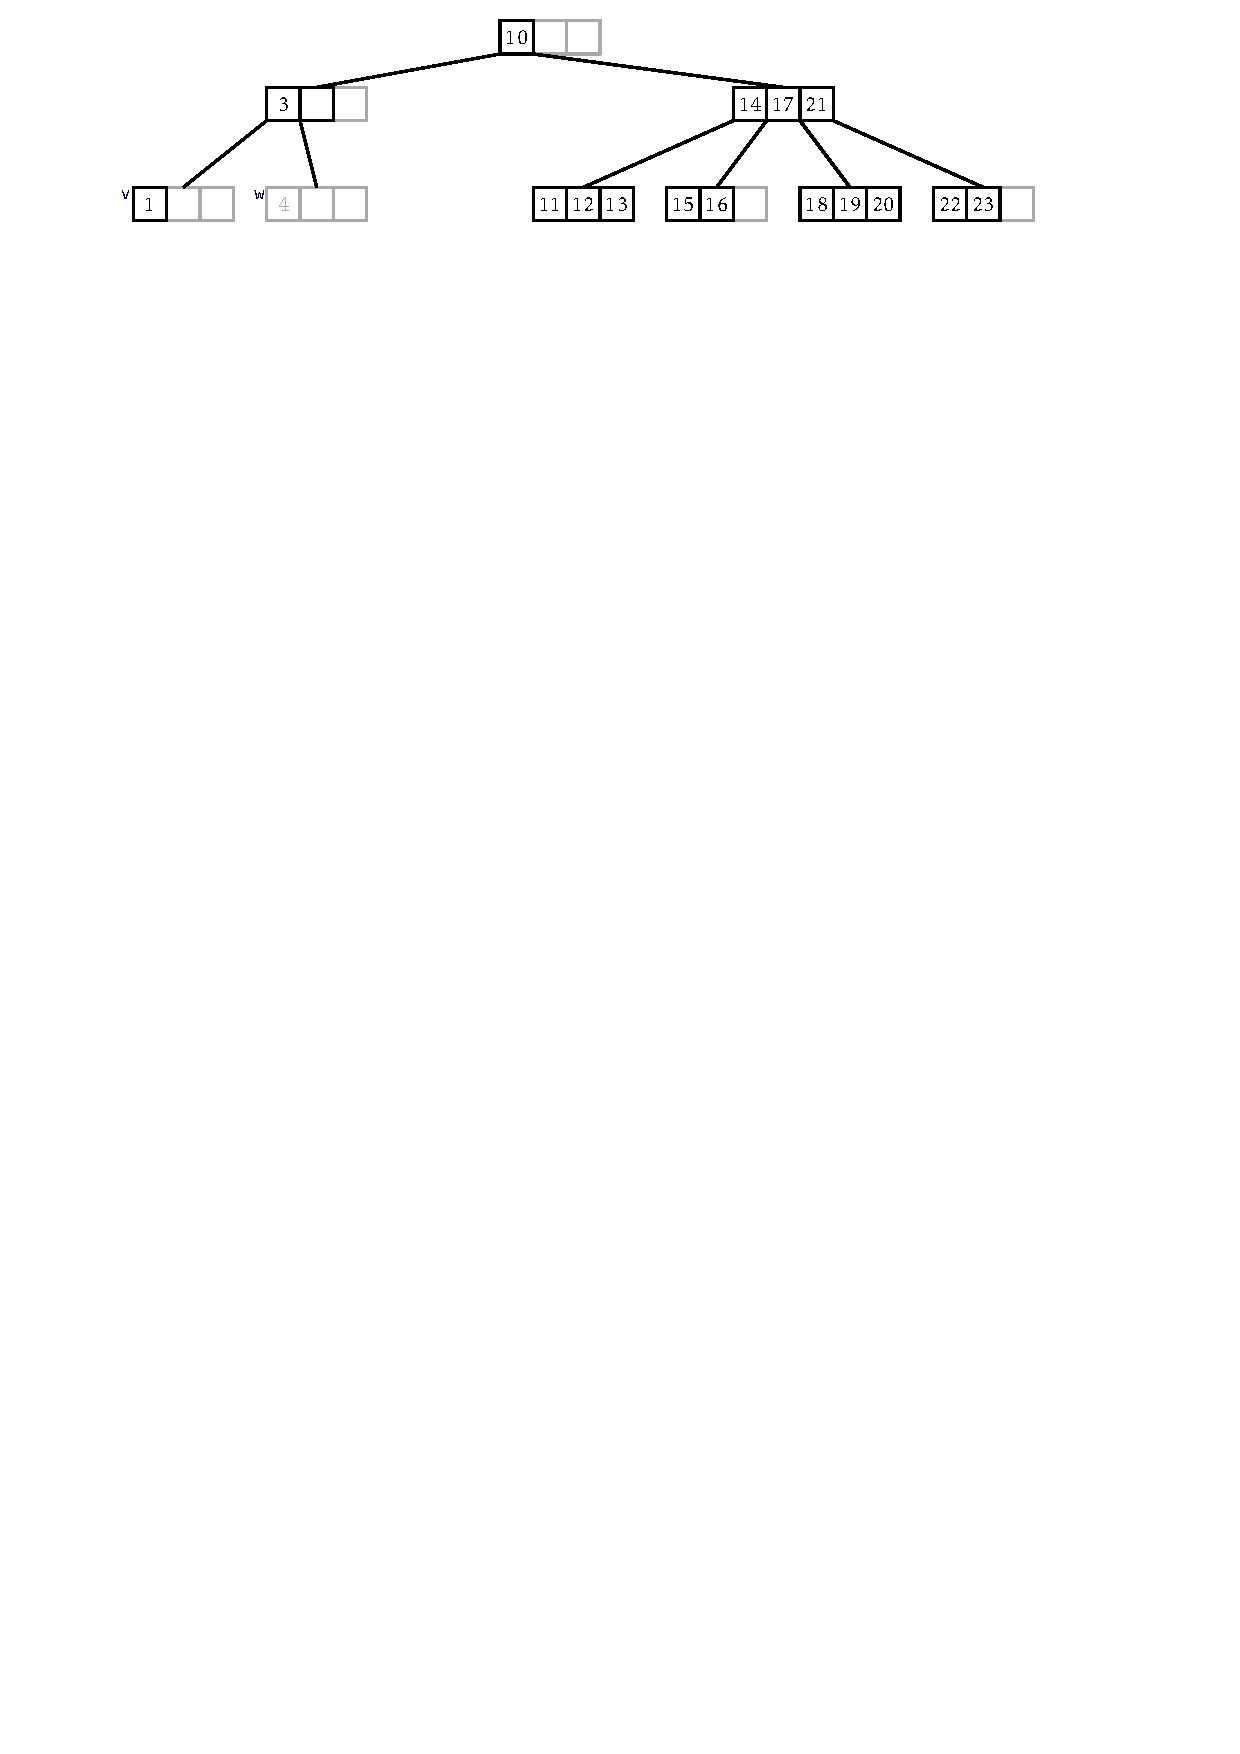
\includegraphics[width=\ScaleIfNeeded]{figs/btree-remove-full-2} \\[2ex]
     \multicolumn{1}{c}{#merge(v,w)#} \\
     \multicolumn{1}{c}{$\Downarrow$} \\[2ex]
     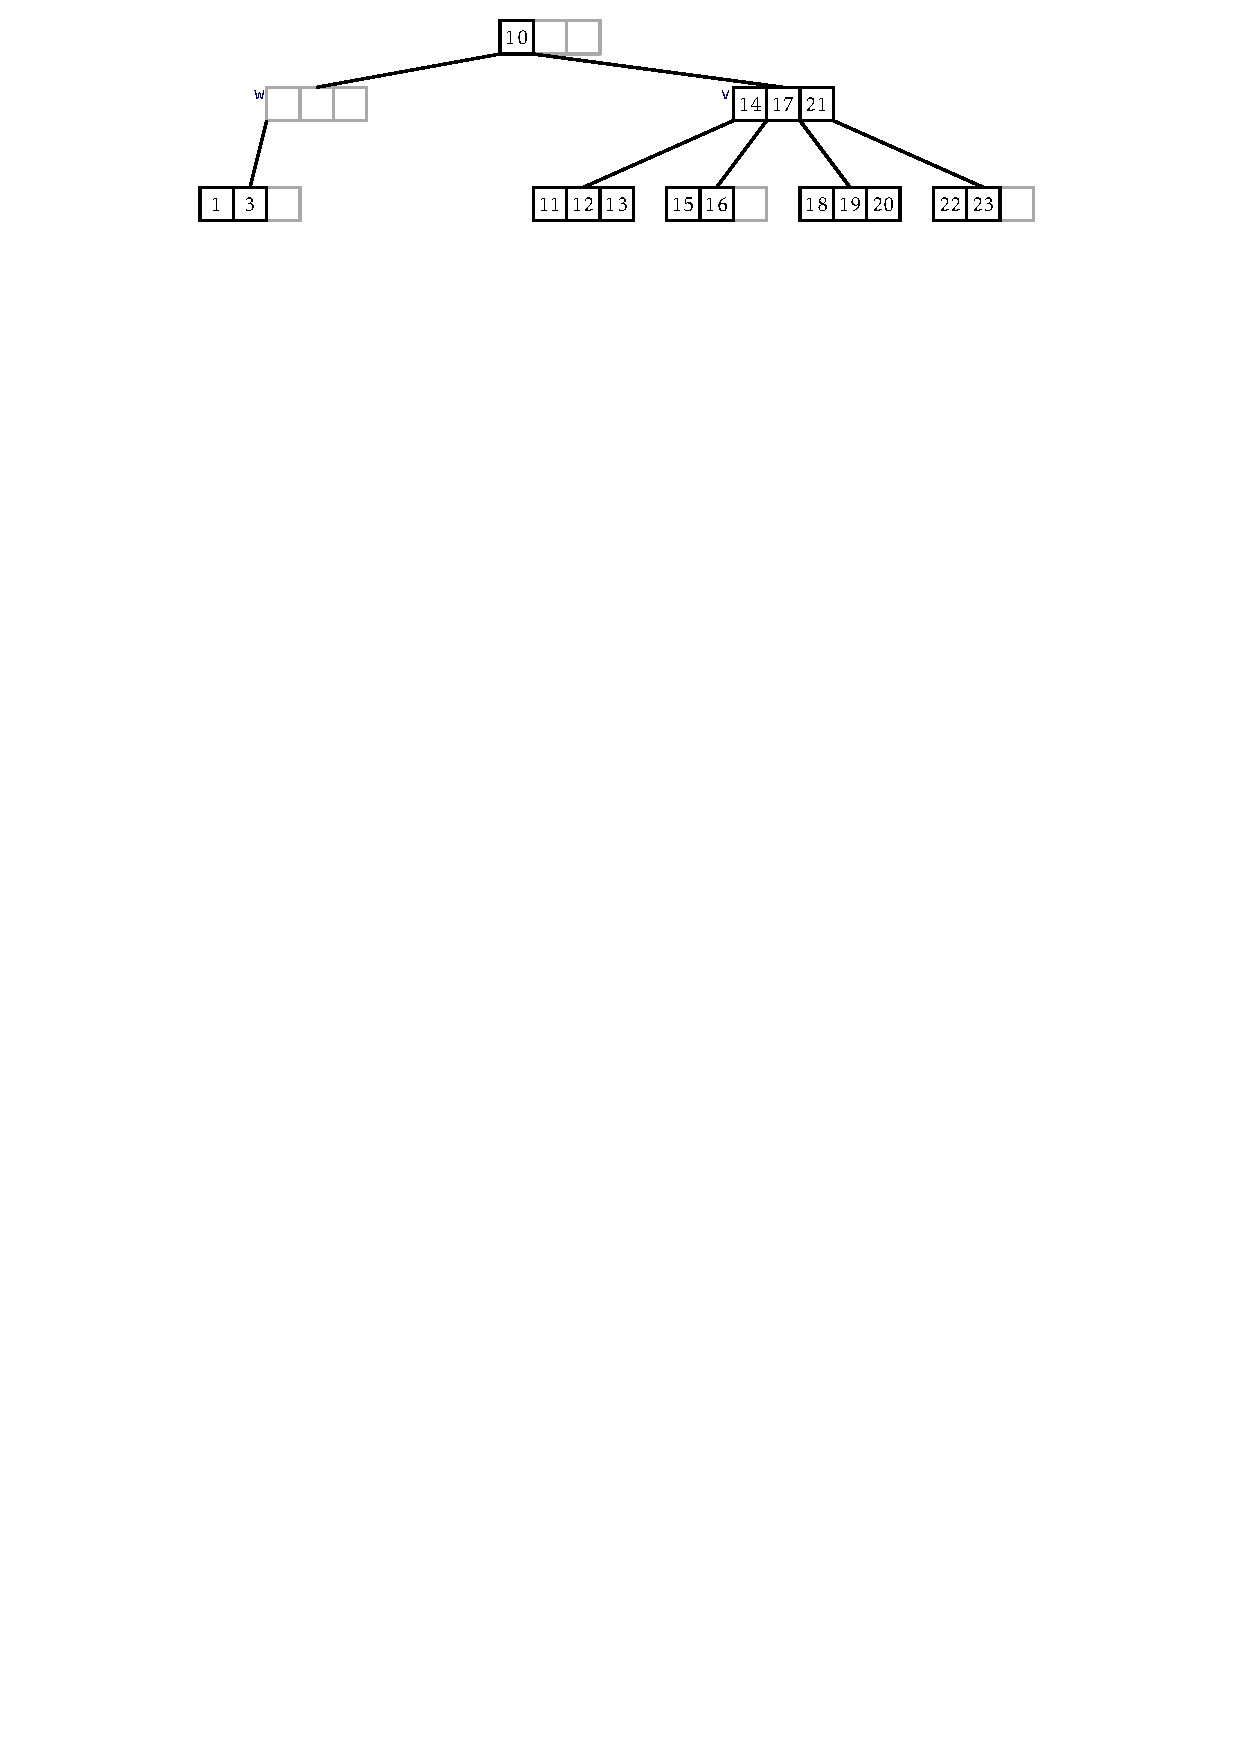
\includegraphics[width=\ScaleIfNeeded]{figs/btree-remove-full-3} \\[2ex]
     \multicolumn{1}{c}{#shiftLR(w,v)#} \\
     \multicolumn{1}{c}{$\Downarrow$} \\[2ex]
     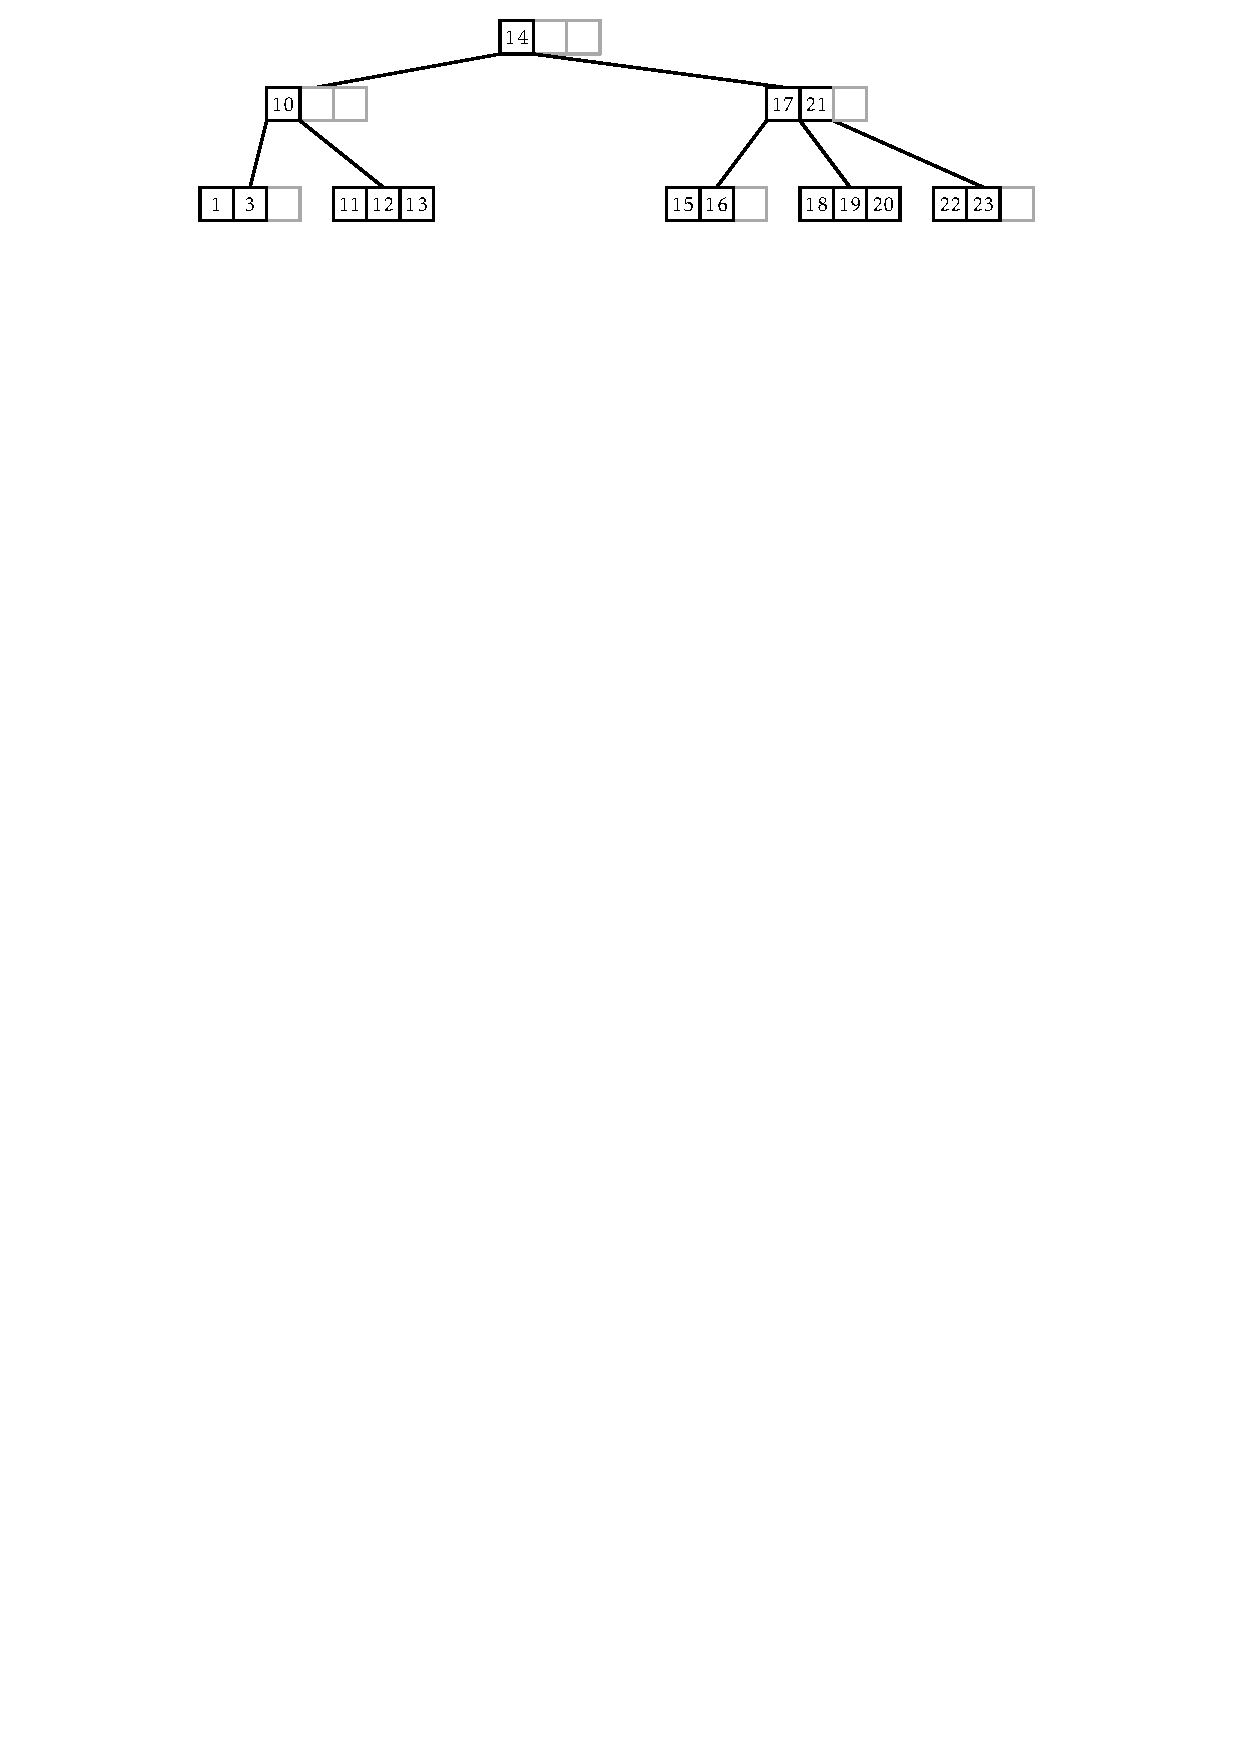
\includegraphics[width=\ScaleIfNeeded]{figs/btree-remove-full-4} \\[2ex]
   \end{tabular}}
   \caption[Removrndo de uma árvore $B$]{Remover o valor 4 de uma árvore $B$ resulta em uma fusão e uma operação de empréstimo.}
   \figlabel{btree-remove-full}
\end{figure}

Quando ocorre um estouro negativo (underflow), #u# pega as chaves emprestadas ou é mesclado com um de seus irmãos. Se #u# for mesclado com um irmão, o pai de #u# agora terá um filho a menos e uma chave a menos, o que pode fazer com que o pai de #u# entre em \emph{underflow}; isso é corrigido novamente pedindo emprestado ou mesclando, mas a mesclagem pode fazer com que o avô de # u # fique em \emph{underflow}. Esse processo retorna à raiz até que não haja mais \emph{underflow} ou até que a raiz tenha seus dois últimos filhos mesclados em um único filho.
Quando ocorre o último caso, a raiz é removida e seu filho único se torna a nova raiz.

A seguir, nos aprofundamos nos detalhes de como cada uma dessas etapas é implementada.
A primeira tarefa do método #remove(x)# é encontrar o elemento #x# que deve ser removido. Se #x# for encontrado em uma folha, então #x# será removido dessa folha. Caso contrário, se #x# for encontrado em #u.keys[i]# para algum nó interno, #u#, então o algoritmo remove o menor valor, #x'#, na subárvore enraizada em #u.children[i+1]#. O valor #x'# é o menor valor armazenado na #BTree# que é maior que #x#. O valor de #x'# é então usado para substituir #x# em #u.keys[i]#. Este processo é ilustrado na \figref{btree-remove}.

\begin{figure}
   \centering{\begin{tabular}{@{}l@{}}
     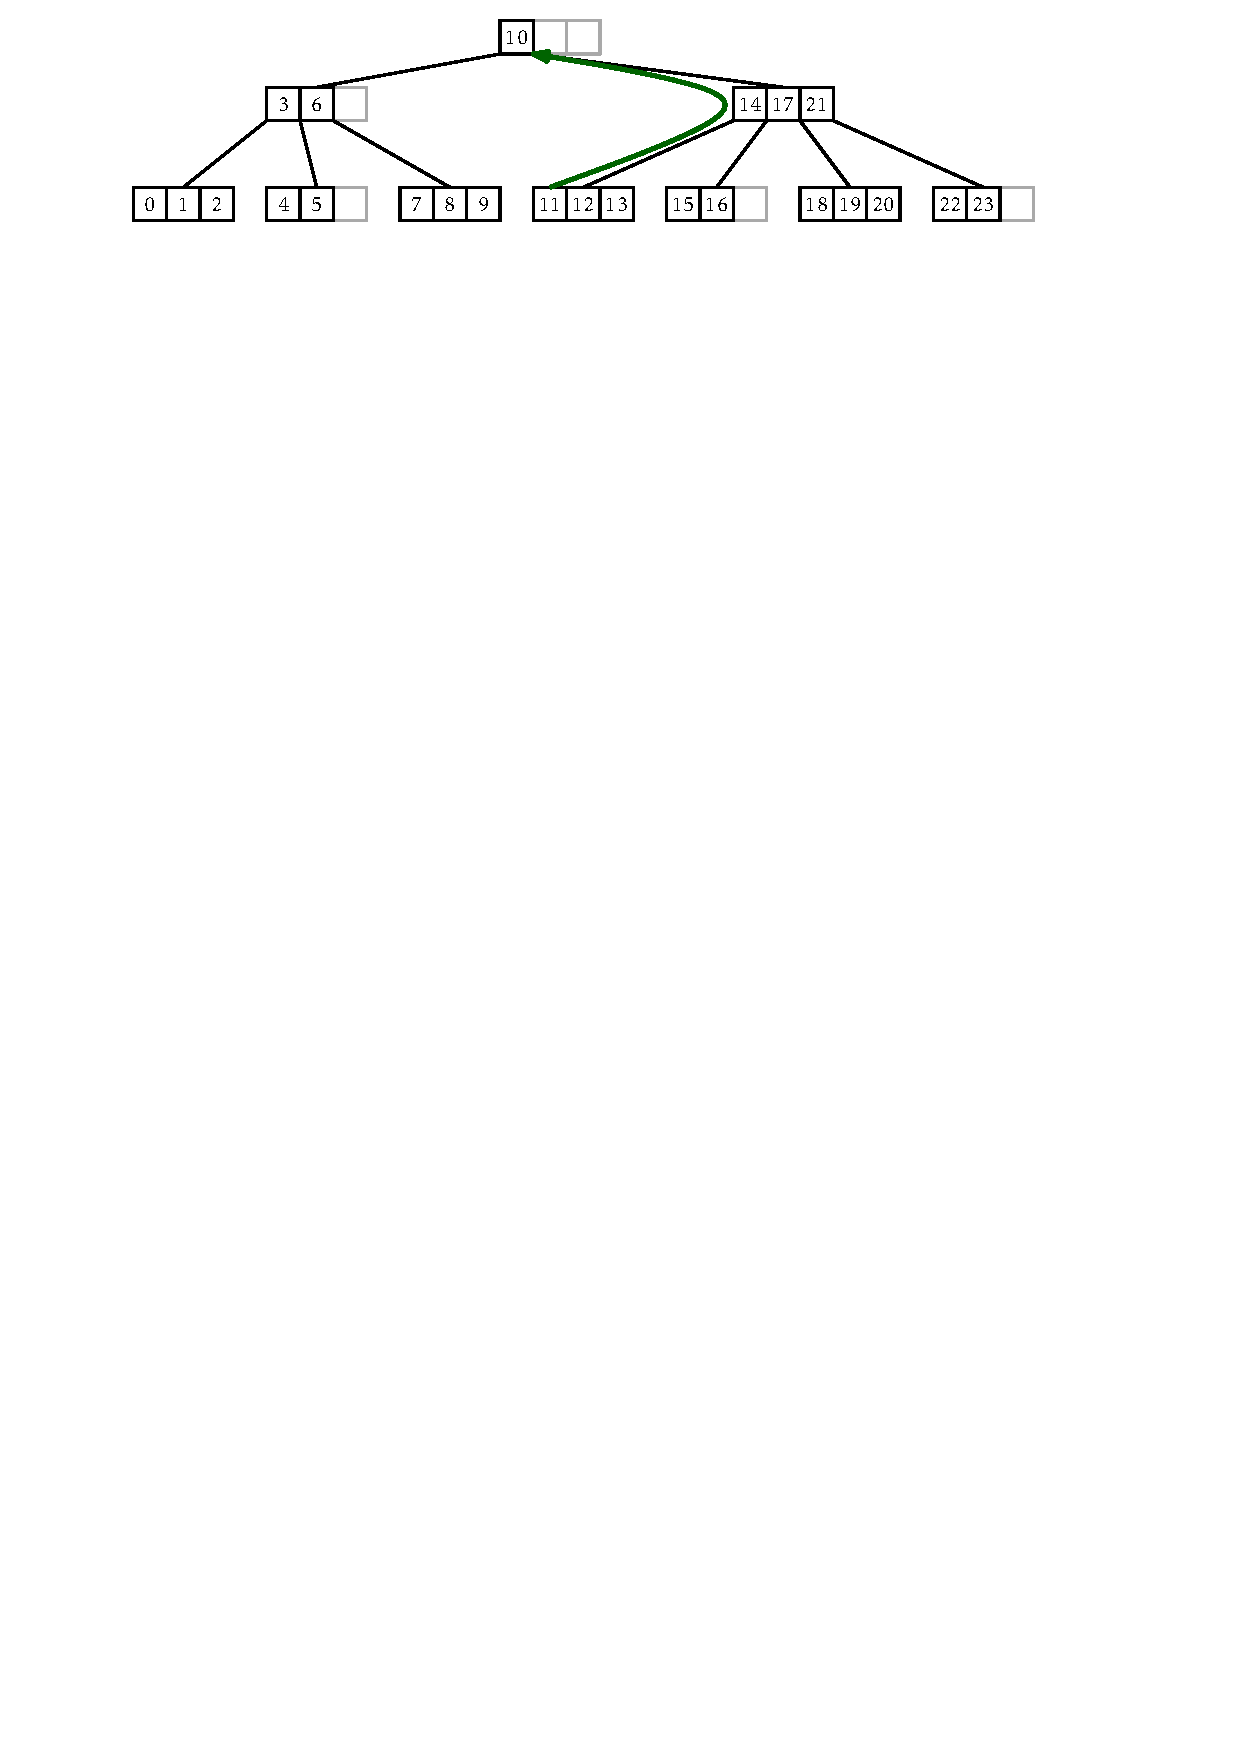
\includegraphics[width=\ScaleIfNeeded]{figs/btree-remove-1} \\[2ex]
     \multicolumn{1}{c}{$\Downarrow$} \\[2ex]
     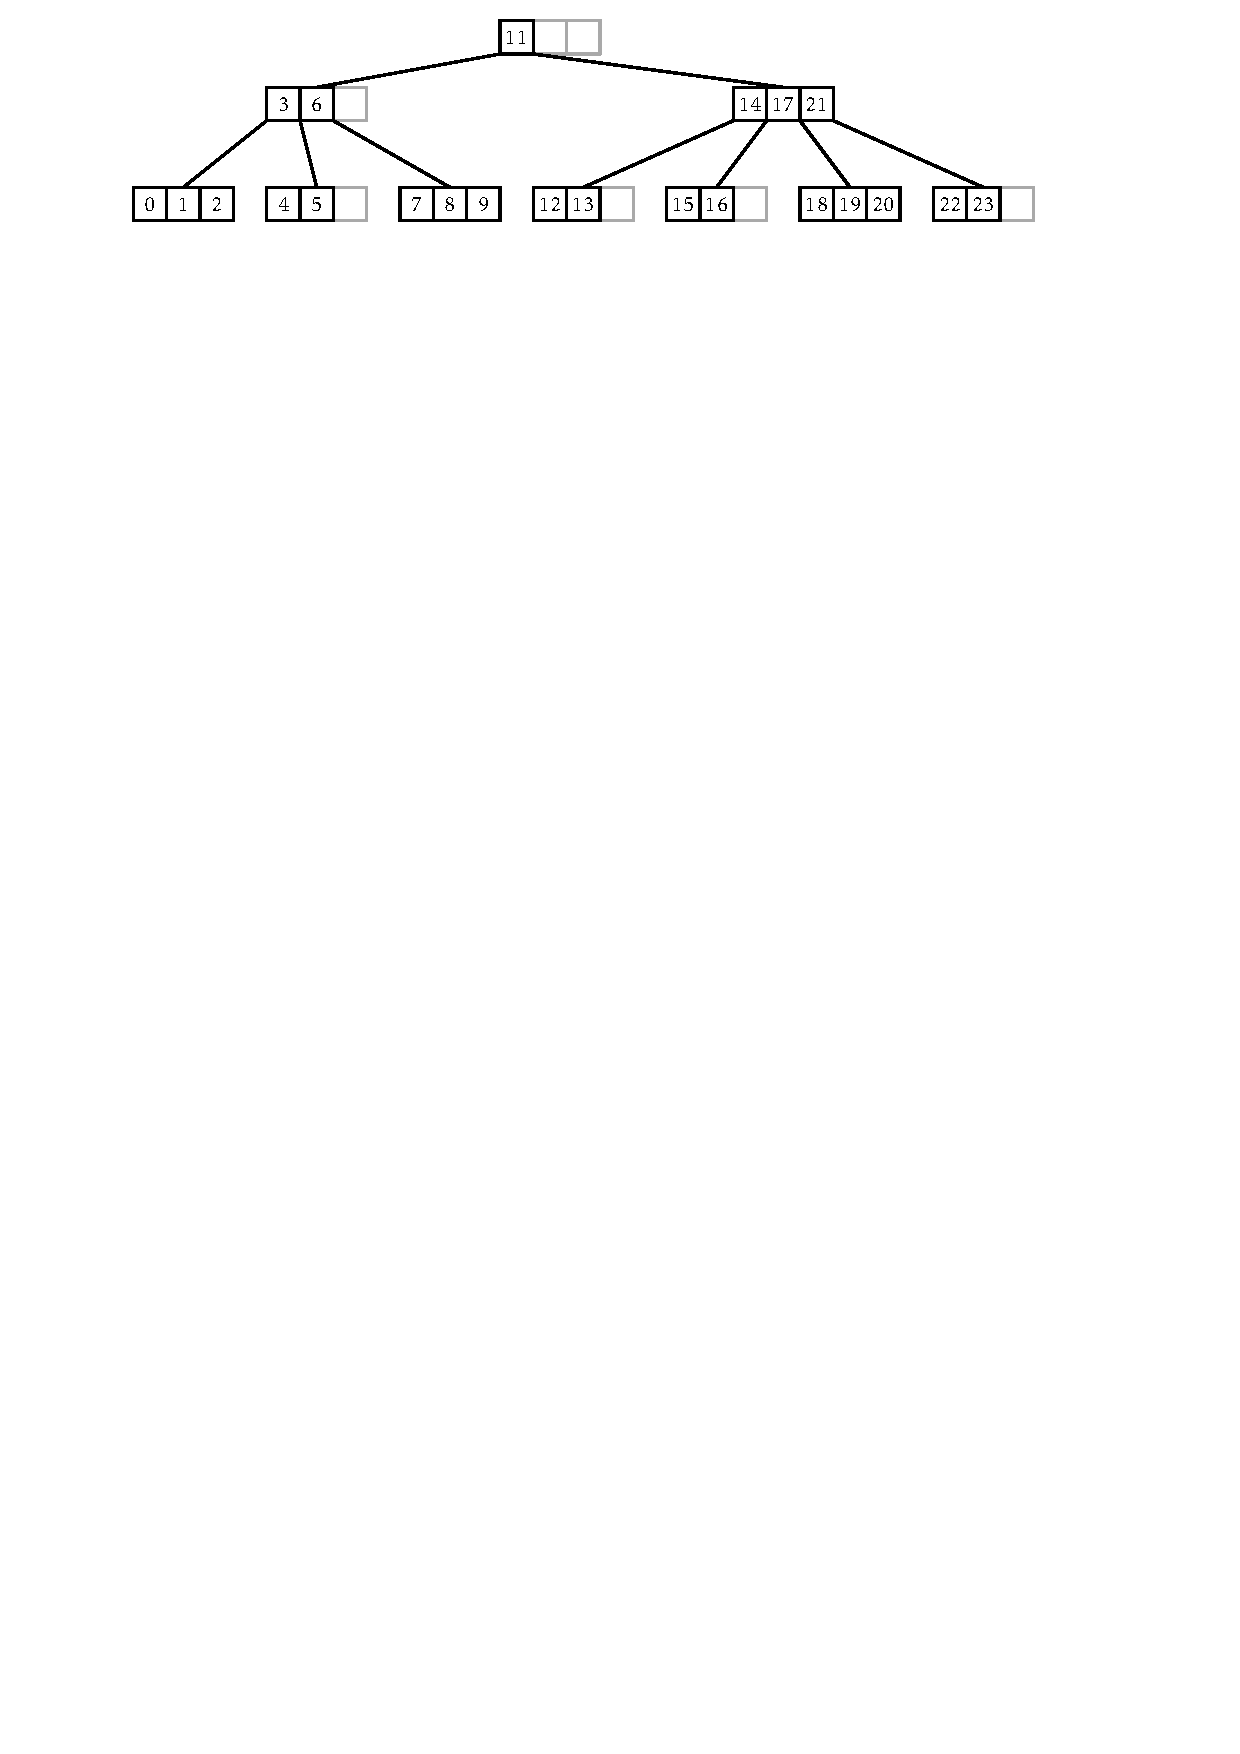
\includegraphics[width=\ScaleIfNeeded]{figs/btree-remove-2} 
   \end{tabular}}
   \caption[A operação de remoção em uma árvore $B$] {A operação #remove(x)# em uma #BTree#. Para remover o valor $#x#=10$, nós o substituímos pelo valor $#x'#=11$ e removemos 11 da folha que o contém.}
   \figlabel{btree-remove}
\end{figure}

O método #removeRecursive(x,ui)# é uma implementação recursiva do algoritmo anterior:
\codeimport{ods/BTree.removeRecursive(x,ui).removeSmallest(ui)}

Observe que, após remover recursivamente o valor #x# do #i#-ésimo filho de #u#, #removeRecursive(x,ui)# precisa garantir que esse filho ainda tenha pelo menos $B-1$ chaves. No código anterior, isso é feito usando um
método chamado #checkUnderflow(x,i)#, que verifica e corrige um estouro negativo no #i#-ésimo filho de #u#. Seja #w# o #i#-ésimo filho de #u#.
Se #w# tiver apenas chaves $B-2$, isso precisa ser corrigido. A correção requer o uso de um irmão de #w#. Pode ser o filho $#i#+1$ de #u# ou o filho $#i#-1$ de #u#. Normalmente usaremos o filho $#i#-1$ de #u#, que é o irmão, #v#, de #w# diretamente à sua esquerda. A única vez que isso não funciona é quando $#i#=0$, caso em que usamos o irmão diretamente  à direita de #w#.
\codeimport{ods/BTree.checkUnderflow(u,i)}
A seguir, nos concentramos no caso em que $#i#\neq 0$ de modo que qualquer underflow no #i#-ésimo filho de #u# seja corrigido com a ajuda do filho $(#i#-1)$  de #u#. O caso $#i#=0$ é semelhante e os detalhes podem ser encontrados no código-fonte que o acompanha.

Para corrigir um estouro negativo no nó #w#, precisamos encontrar mais chaves (e possivelmente também filhos), para #w#. Existem duas maneiras de fazer isso:

\begin{description}
  \item[Pedindo emprestado:]
  \index{empréstimo}%
  Se #w# tiver um irmão, #v#, com mais de $B-1$ chaves, então #w# pode emprestar algumas chaves (e possivelmente também filhos) de #v#.
  Mais especificamente, se #v# armazena #size(v)# chaves, então, entre elas, #v# e #w# têm um total de
  \[
     B-2 + #size(w)# \ge 2B-2
  \]
  chaves. Podemos, portanto, mudar as chaves de #v# para #w# de modo que cada um de #v# e #w# tenha pelo menos $B-1$ chaves. Este processo é ilustrado na
  \figref{btree-borrow}.

  \begin{figure}
      \centering{\begin{tabular}{@{}l@{}}
       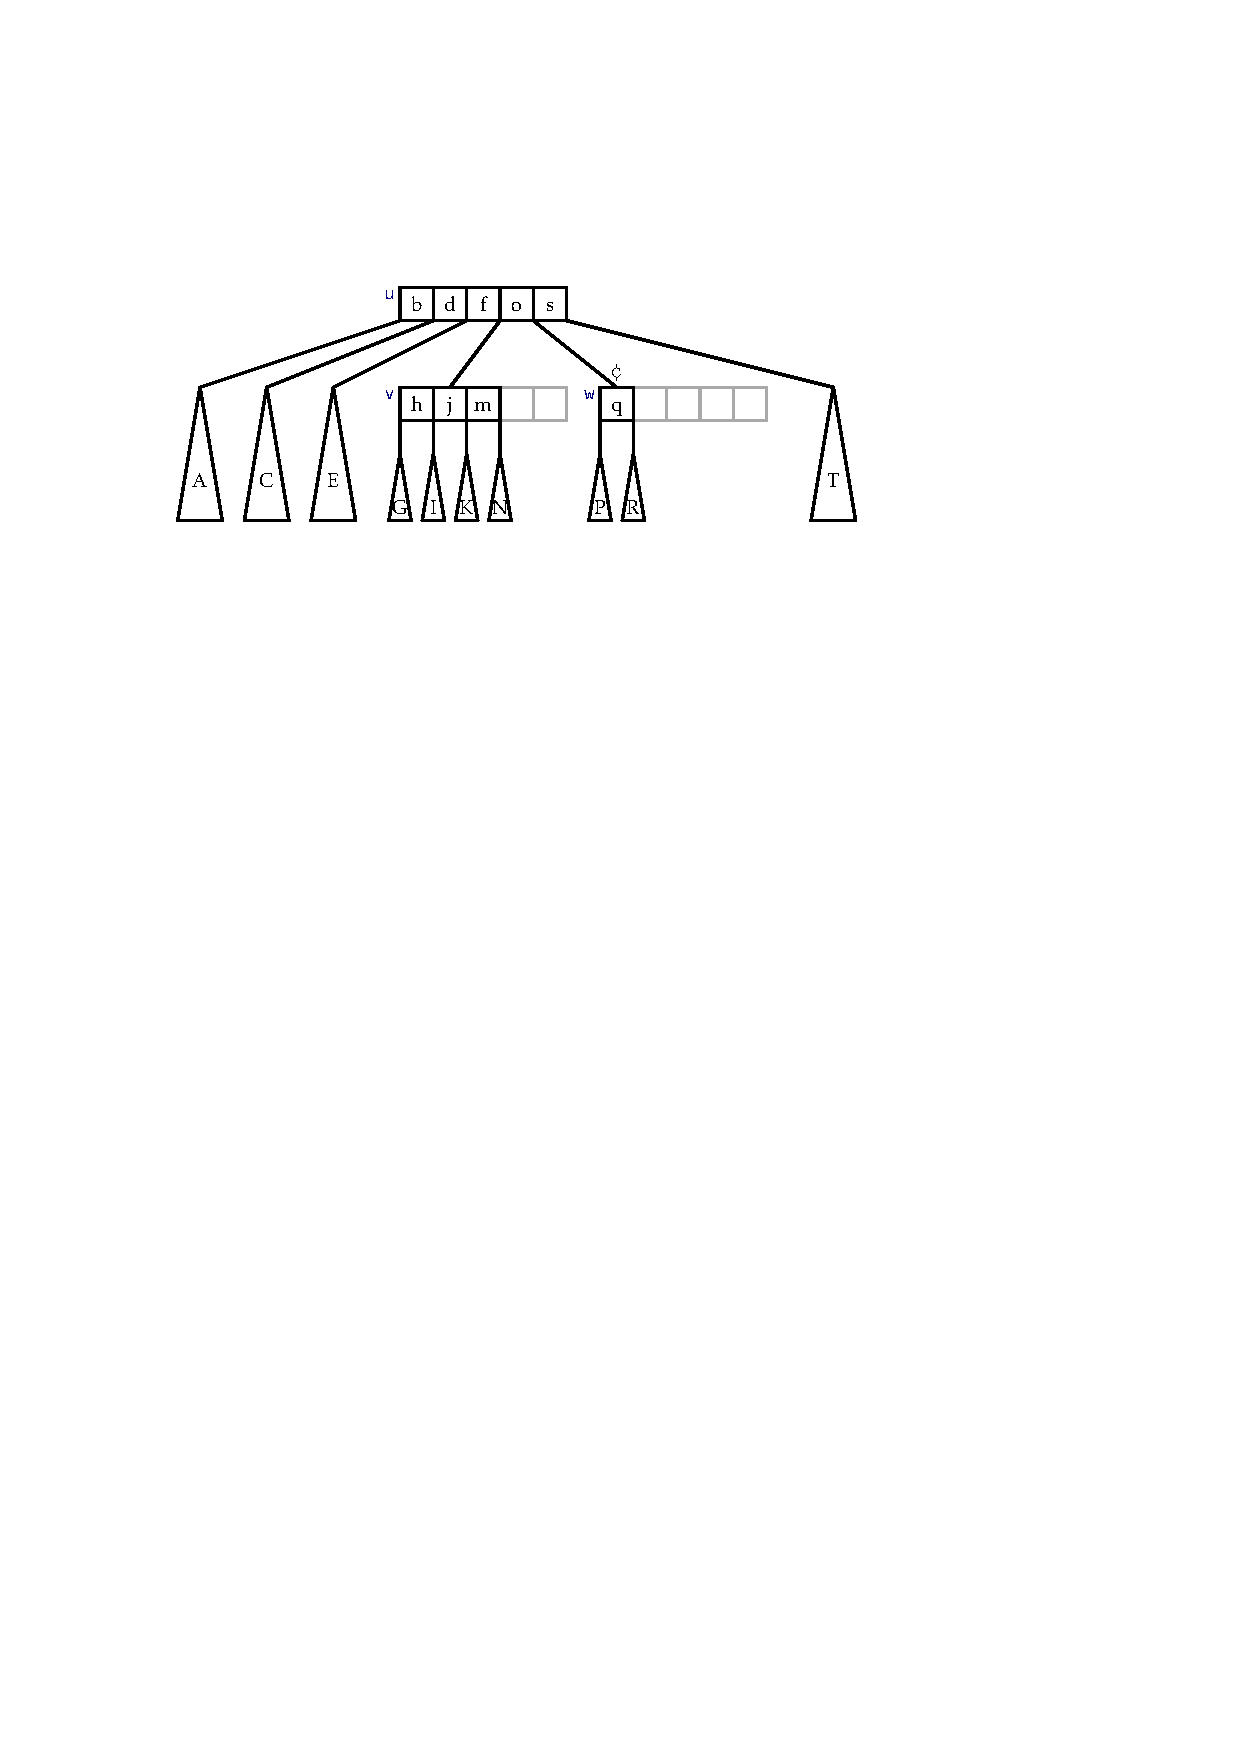
\includegraphics[width=\ScaleIfNeeded]{figs/btree-borrow-1} \\[2ex]
       \multicolumn{1}{c}{#shiftRL(v,w)#} \\ 
       \multicolumn{1}{c}{$\Downarrow$} \\[2ex]
       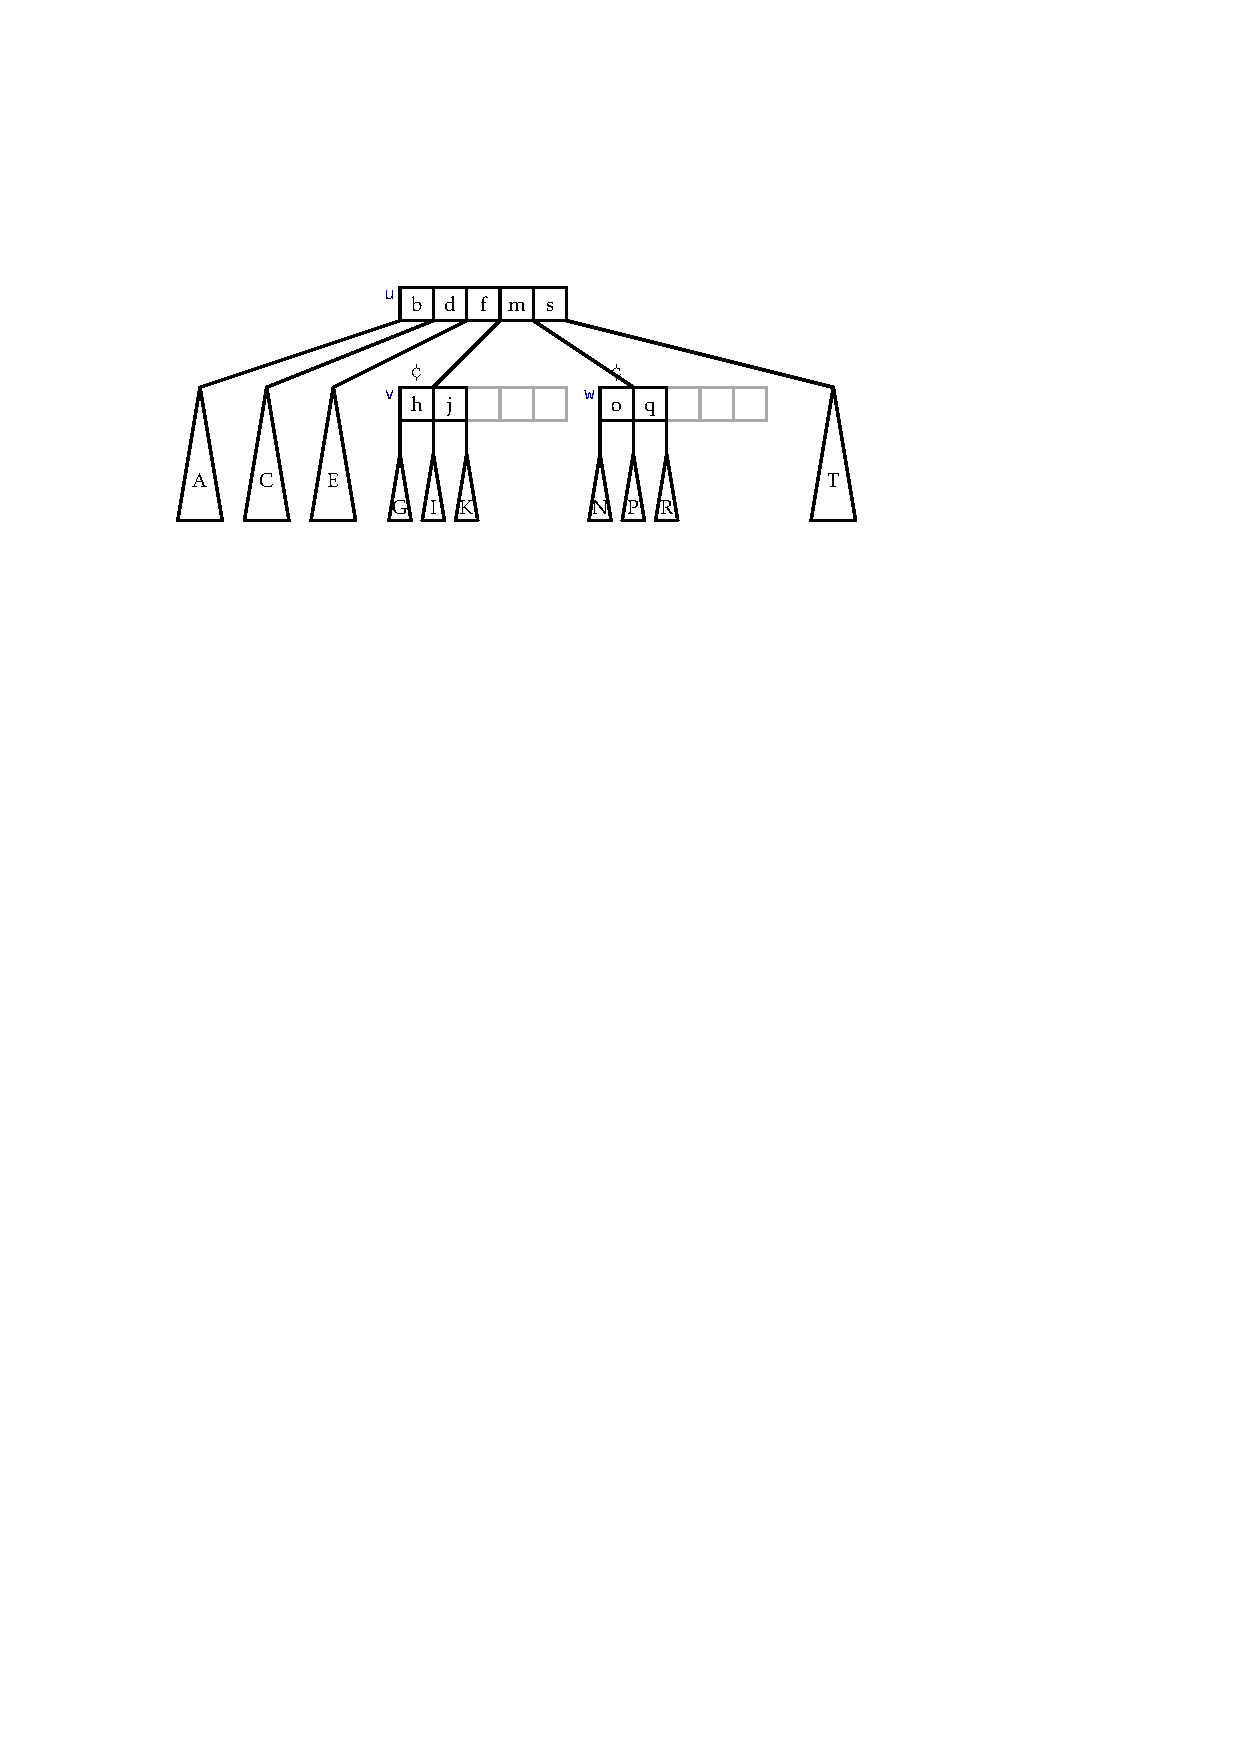
\includegraphics[width=\ScaleIfNeeded]{figs/btree-borrow-2} \\
     \end{tabular}}
    \caption[Emprestando em uma árvore de $B$]{Se #v# tem mais que $B-1$ chaves,
       então #w# pedir chaves emprestado a #v#.}
    \figlabel{btree-borrow}
  \end{figure}
  
  \item[Mesclando:]
  \index{merge}%
  Se #v# tiver apenas chaves $B-1$, devemos fazer algo mais drástico, já que #v# não pode se dar ao luxo de fornecer chaves para #w#. Portanto, \emph{mesclamos} #v# e #w# como mostrado na \figref{btree-merge}. A operação de mesclagem é o oposto da operação de divisão. Ele pega dois nós que contêm um total de $2B-3$ chaves e os mescla em um único nó que contém $2B-2$ chaves. (A chave adicional vem do  fato de que, quando mesclamos #v# e #w#, seu pai comum, #u#, agora tem um filho a menos e, portanto, precisa desistir de uma de suas chaves.)
  
  \begin{figure}
     \centering{\begin{tabular}{@{}l@{}}
       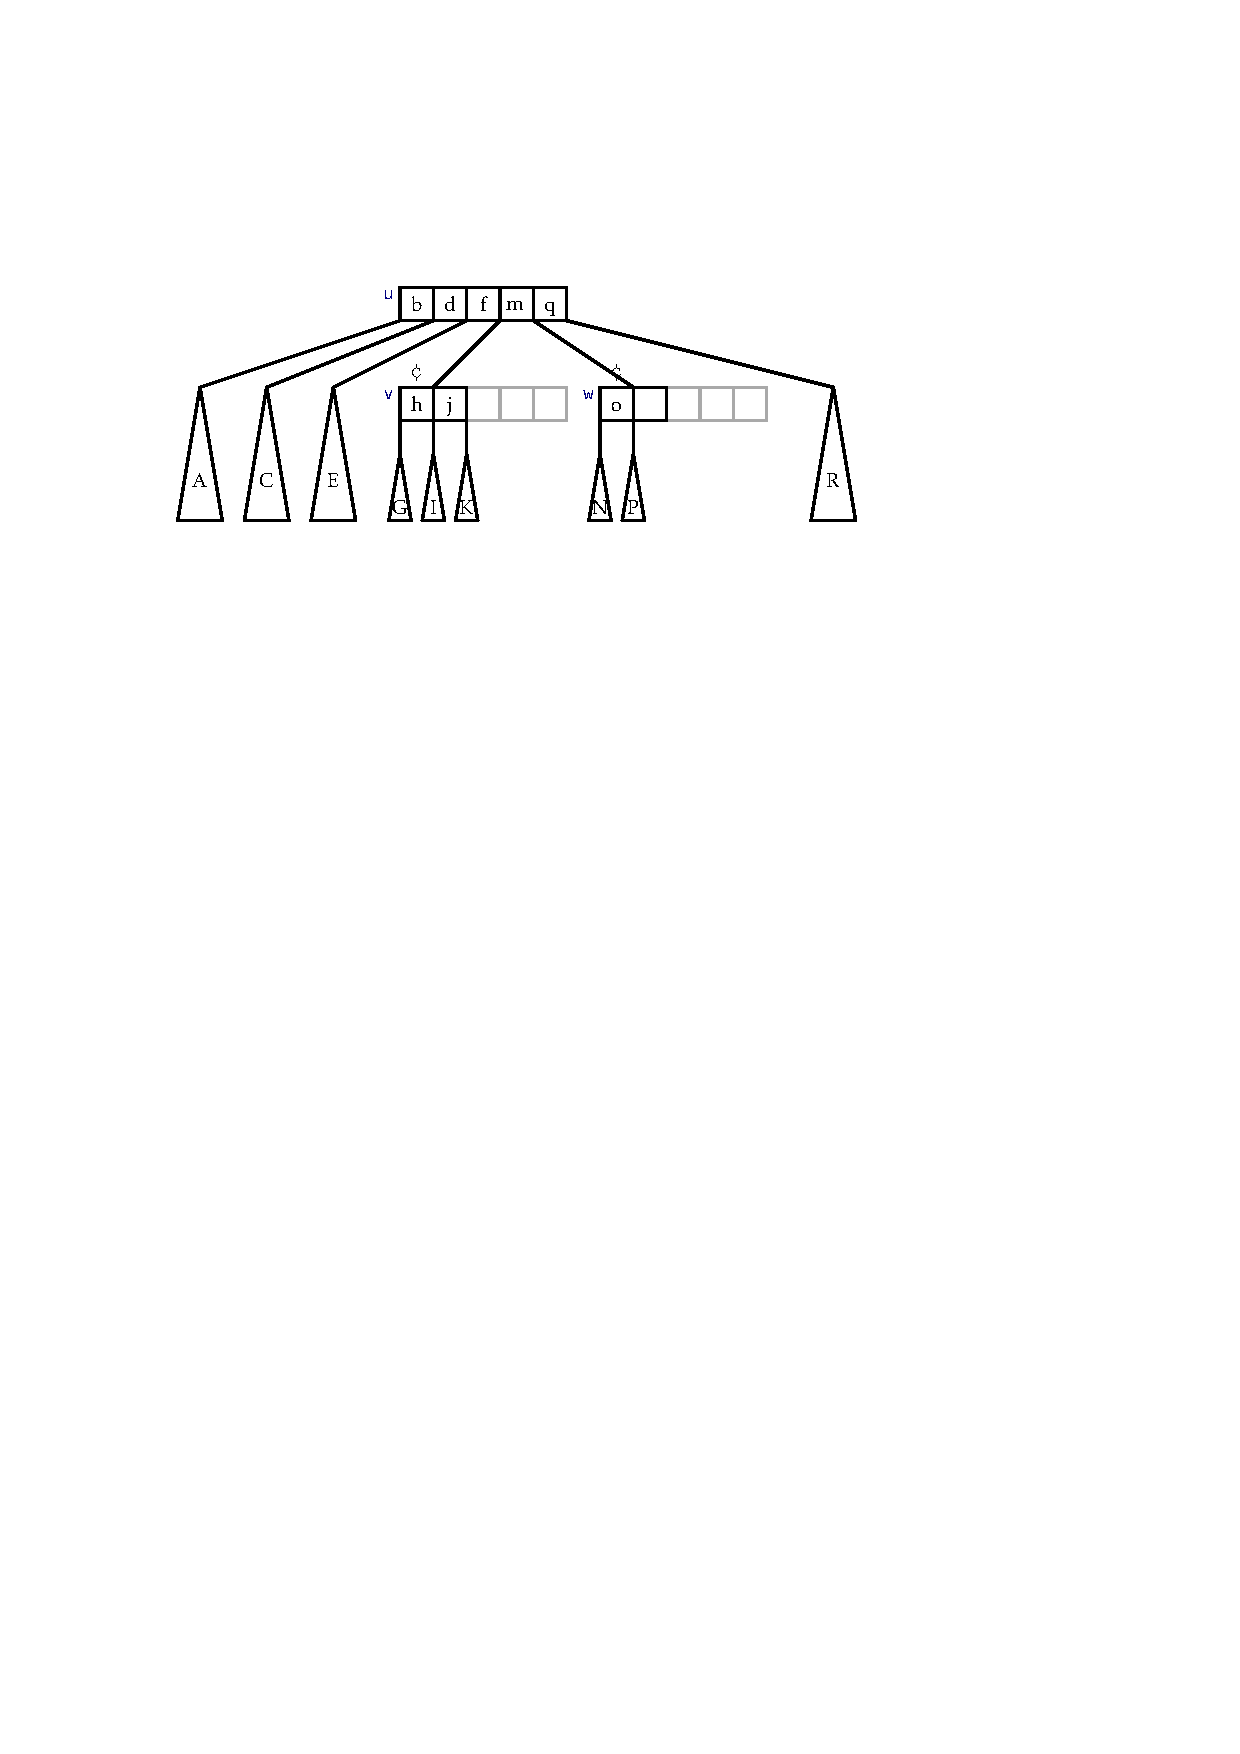
\includegraphics[width=\ScaleIfNeeded]{figs/btree-merge-1} \\[2ex]
       \multicolumn{1}{c}{#merge(v,w)#} \\ 
       \multicolumn{1}{c}{$\Downarrow$} \\[2ex]
       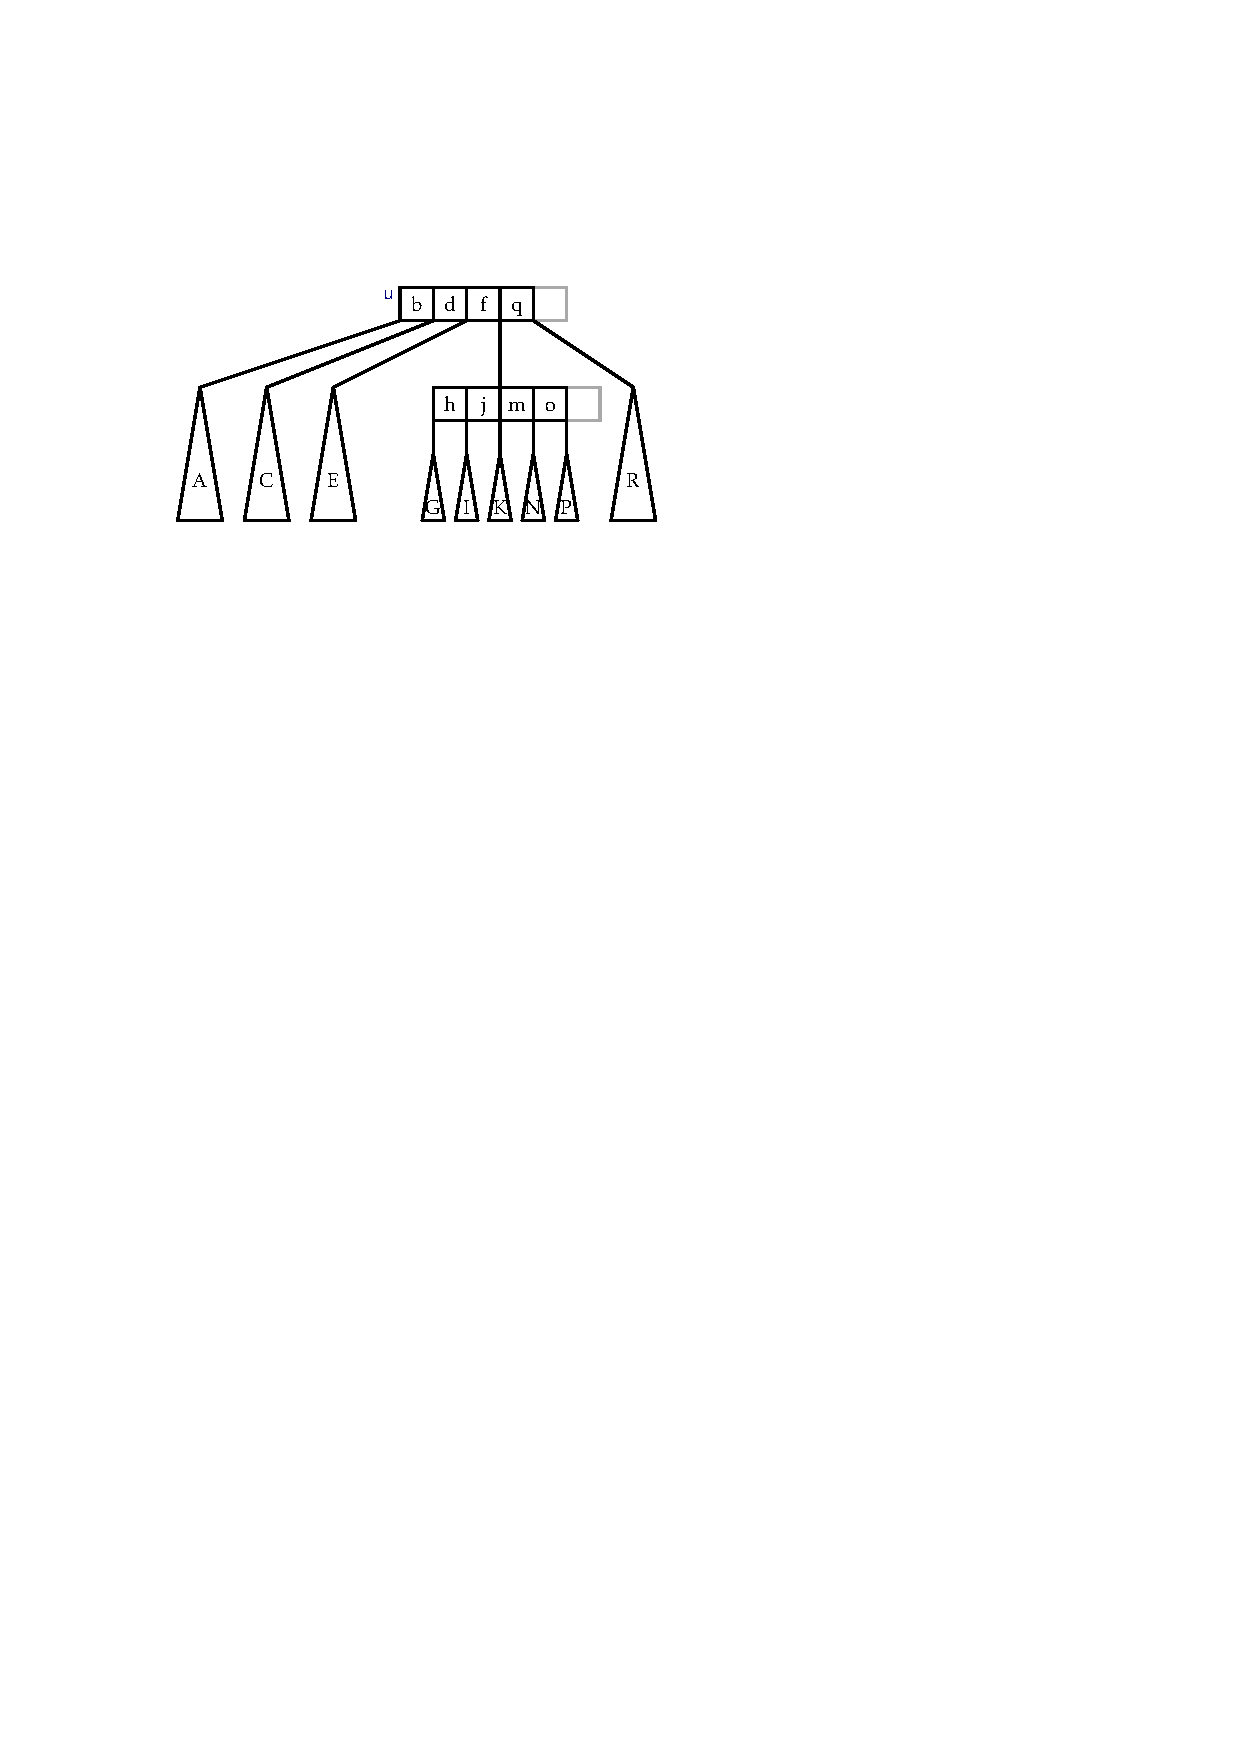
\includegraphics[width=\ScaleIfNeeded]{figs/btree-merge-2} \\
     \end{tabular}}
     \caption[Mesclagem em uma árvore $B$]{Mesclando dois irmãos #v# e #w# em uma árvore $B$ ($B=3$).}
     \figlabel{btree-merge}
  \end{figure}
\end{description}

\codeimport{ods/BTree.checkUnderflowNonZero(u,i).checkUnderflowZero(u,i)}

Para resumir, o método #remove(x)# em uma árvore $B$ segue um caminho da raiz para a folha, remove uma chave #x'# de uma folha, #u# e, em seguida, executa zero ou mais operações de mesclagem envolvendo #u# e seus ancestrais e executa no máximo uma operação de empréstimo. Como cada operação de mesclagem e empréstimo envolve a modificação de apenas três nós, e apenas $O(\log_B #n#)$ dessas operações ocorrem, todo o processo leva um tempo $O(\log_B #n#)$ no modelo de memória externa. Novamente, no entanto, cada operação de mesclagem e empréstimo leva um tempo $O(B)$ no modelo de palavra-RAM, então (por enquanto) o máximo que podemos dizer sobre o tempo de execução exigido por #remove(x)# no modelo de palavra-RAM é $ O(B\log_B #n#)$.

\subsection{Análise Amortizada de Árvores $B$}
\seclabel{btree-amortized}

Até agora, mostramos que
\begin{enumerate}
  \item No modelo de memória externa, o tempo de execução de #find(x)#, #add(x)# e #remove(x)# em uma árvore $B$ é $O(\log_B #n#)$.
  \item No modelo palavra-RAM, o tempo de execução de #find(x)# é $O(\log #n#)$ e o tempo de execução de #add(x)# e #remove(x)# é $O(B\log #n#)$.
\end{enumerate}

O seguinte lema mostra que, até agora, superestimamos o número de operações de mesclagem e divisão realizadas por árvores $B$.

\begin{lem}\lemlabel{btree-split}
  Começar com uma árvore $B$ vazia e executar qualquer sequência de $m$ operações  #add(x)# e #remove(x)# resulta em no máximo $3m/2$ divisões, mesclagens e empréstimos sendo executados.
\end{lem}

\begin{proof}
   A prova disso já foi esboçada em
   \secref{redblack-summary} para o caso especial em que $B=2$.
   O lema pode ser comprovado usando um esquema de crédito,
   \index{esquema de crédito}%
   no qual
  \begin{enumerate}
    \item cada operação de divisão, fusão ou empréstimo é paga com dois créditos, ou seja, um crédito é retirado cada vez que uma dessas operações ocorre; e
    \item no máximo três créditos são criados durante qualquer operação #add(x)# ou #remove(x)#.
  \end{enumerate}
  Como no máximo $3m$ créditos são criados e cada divisão, fusão e empréstimo é pago com dois créditos, segue-se que no máximo $3m/2$ de divisões, fusões e empréstimos são realizados.
  Esses créditos são ilustrados usando o símbolo \cent\ nas Figuras~\ref{fig:btree-split}, \ref{fig:btree-borrow}, e
  \ref{fig:btree-merge}.

  Para acompanhar esses créditos, a prova mantém o seguinte 
  \emph {invariante de crédito}:
  \index{invariante de crédito}%
  Qualquer nó não raiz com $B-1$ chaves  armazena um crédito e qualquer nó com $2B-1$ chaves  armazena três créditos. Um nó que armazena pelo menos $B$ chaves e a maioria das $2B-2$ chaves  não precisa armazenar nenhum crédito. O que falta é mostrar que podemos manter a invariante de crédito e satisfazer as propriedades 1 e 2, acima, durante cada operação #add(x)# e #remove(x)#.

  \paragraph{Adicionando:}
  O método #add(x)# não realiza mesclagens ou empréstimos, portanto, precisamos apenas considerar as operações de divisão que ocorrem como resultado de chamadas para #add(x)#.

  Cada operação de divisão ocorre porque uma chave é adicionada a um nó, #u#, que já contém $2B-1$ chaves. Quando isso acontece, #u# é dividido em dois nós, #u'# e #u''# tendo $B-1$ e $B$ chaves, respectivamente. Antes desta operação, #u# estava armazenando $2B-1$ chaves  e, portanto, três créditos.
  Dois desses créditos podem ser usados para pagar a divisão e o outro crédito pode ser dado a #u'# (que tem $B-1$ chaves) para manter a invariante de crédito. Portanto, podemos pagar pela divisão e manter a invariante de crédito durante qualquer divisão.

  A única outra modificação nos nós que ocorre durante uma operação #add(x)# ocorre depois que todas as divisões, se houver, forem concluídas. Esta modificação envolve a adição de uma nova chave a algum nó #u'#. Se, antes disso, #u'# tinha $2B-2$ filhos, agora tem $2B-1$ filhos e deve, portanto, receber três créditos. Estes são os únicos créditos dados pelo método #add(x)#.

  \paragraph{Removendo:}
  Durante uma chamada para #remove(x)#, zero ou mais mesclagens ocorrem e são possivelmente seguidas por um único empréstimo. Cada mesclagem ocorre porque dois nós, #v# e #w#, cada um dos quais tinha exatamente $B-1$ chaves antes de chamar #remove(x)#, foram mesclados em um único nó com exatamente $2B-2$ chaves.
  Cada mesclagem, portanto, libera dois créditos que podem ser usados para pagar pela fusão.

  Depois que quaisquer fusões são realizadas, no máximo uma operação de empréstimo ocorre, após a qual não ocorrem mais fusões ou empréstimos. Esta operação de empréstimo ocorre apenas se removermos uma chave de uma folha, #v#, que possui $B-1$ chaves.
  O nó #v#, portanto, tem um crédito, e esse crédito vai para o custo do empréstimo. Esse único crédito não é suficiente para pagar o empréstimo, então criamos um crédito para completar o pagamento.

  Neste ponto, criamos um crédito e ainda precisamos mostrar que a invariante de crédito pode ser mantida. No pior caso, o irmão de #v#, #w#, tem exatamente $B$ chaves antes do empréstimo, de forma que, depois, tanto #v# quanto #w# têm $B-1$ chaves. Isso significa que #v# e #w# cada um deve armazenar um crédito quando a operação for concluída.
  Portanto, neste caso, criamos dois créditos adicionais para dar a #v# e #w#. Como um empréstimo acontece no máximo uma vez durante uma operação #remove(x)#, isso significa que criamos no máximo três créditos, conforme necessário.

  Se a operação #remove(x)# não inclui uma operação de empréstimo, é porque termina removendo uma chave de algum nó que, antes da operação, tinha $B$ ou mais chaves. No pior caso, este nó tinha exatamente $B$ chaves, de modo que agora tem $B-1$ chaves  e deve receber um crédito, que criamos.

  Em ambos os casos --- quer a remoção termine com uma operação de empréstimo ou não --- no máximo três créditos precisam ser criados durante uma chamada para #remove(x)# para manter a invariante de crédito e pagar por todos os empréstimos e mesclagens que ocorrer. Isso completa a prova do lema.
\end{proof}

O objetivo de \lemref{btree-split} é mostrar que, no modelo de palavra-RAM, o custo de divisões, fusões e junções durante uma sequência de $m$ operações #add(x)# e #remove(x)#  é apenas $O(Bm)$. Ou seja, o custo amortizado por operação é apenas $O(B)$, então o custo amortizado de #add(x)# e #remove(x)# no modelo de palavra-RAM é $O(B+\log #n#)$.
Isso é resumido pelo seguinte par de teoremas:

\begin{thm}[Árvore $B$ em Memória Externa]
  Uma #BTree# implementa a interface #SSet#. No modelo de memória externa, uma #BTree# suporta as operações #add(x)#, #remove(x)# e #find(x)# com tempo $O(\log_B #n#)$ por operação.
\end{thm}

\begin{thm}[Árvores $B$ em Palavra-RAM]
  Uma #BTree# implementa a interface #SSet#. No modelo de palavra-RAM, e ignorando o custo de divisões, fusões e empréstimos, uma #BTree# oferece suporte às operações #add(x)#, #remove(x)# e  #find(x)# em tempo $O(\log #n#)$ por operação.
  Além disso, começando com uma #BTree# vazia, qualquer sequência de $m$ operações #add(x)# e #remove(x)#  resulta em um total de tempo $O(Bm)$ gasto para realizar divisões, fusões e empréstimos.
\end{thm}

\section{Discussão e Exercícios}

O modelo de computação de memória externa foi introduzido por Aggarwal e Vitter \cite{av88}. Às vezes também é chamado de \emph{modelo de E/S}
\index{modelo de E/S}%
ou de \emph{modelo de acesso ao disco}. 
\index{modelo de acesso ao disco}%

As árvores $B$ estão para a pesquisa de memória externa o que as árvores de pesquisa binárias estão para a pesquisa de memória interna. As árvores $B$ foram introduzidos por Bayer e McCreight \cite{bm70} em 1970 e, menos de dez anos depois, o título do artigo da ACM Computing Surveys de Comer referia-se a elas como ubíquas \cite{c79}.

Como árvores de busca binárias, existem muitas variantes de árvores $B$, incluindo árvores $B^+$,
\index{arvore@árvore B+@árvore $B^+$}%
árvores $B^*$,
\index{arvore@árvore B*@árvore $B^*$}%
e árvores contadas $B$.
\index{arvore@árvore contada $B$}%
Árvores $B$ são realmente onipresentes e são a estrutura de dados primária em muitos sistemas de arquivos, incluindo o HFS+ da Apple,
\index{HFS+}%
o NTFS da Microsoft, 
\index{NTFS}%
e o Ext4 do Linux;
\index{Ext4}%
todos os principais sistemas de banco de dados; e armazenamentos de valores-chave usados na computação em nuvem.
A pesquisa recente de Graefe \cite{g10} fornece uma visão geral de mais de 200 páginas de muitos aplicativos modernos, variantes e otimizações de árvores $B$.

Árvores $B$ implementam a interface #SSet#. Se apenas a interface #USet# for necessária, o hashing da memória externa
\index{hashing da memória externa}%
poderia ser usado como uma alternativa às árvores $B$. Existem esquemas de hashing de memória externa; veja, por exemplo, Jensen e Pagh~\cite{jp08}. Esses esquemas implementam as operações #USet# em tempo esperado $O(1)$  no modelo de memória externa. No entanto, por vários motivos, muitos aplicativos ainda usam árvores $B$, embora requeiram apenas operações #USet#.

Uma das razões pelas quais as árvores $B$ são uma escolha tão popular é que frequentemente têm um desempenho melhor do que seus limites de tempo de execução $O(\log_B #n#)$ sugerem. A razão para isso é que, em configurações de memória externa, o valor de $B$ é normalmente muito grande -- na casa das centenas ou mesmo milhares. Isso significa que 99\% ou mesmo 99,9\% dos dados em uma árvore $B$ são armazenados nas folhas. Em um sistema de banco de dados com grande memória, pode ser possível armazenar em cache todos os nós internos de uma árvore $B$ na RAM, pois eles representam apenas 1\% ou 0,1\% do conjunto de dados total. Quando isso acontece, significa que uma busca em uma árvore $B$ envolve uma busca muito rápida na RAM, através dos nós internos, seguida por um único acesso à memória externa para recuperar uma folha.

\begin{exc}
  Mostre o que acontece quando as chaves 1.5 e 7.5 são adicionadas à árvore $B$ na \figref{btree}.
\end{exc}

\begin{exc}
  Mostre o que acontece quando as chaves 3 e 4 são removidas da árvore $B$ na \figref{btree}.
\end{exc}

\begin{exc}
  Qual é o número máximo de nós internos em uma árvore $B$ que armazena #n# chaves (como uma função de #n# e $B$)?
\end{exc}

\begin{exc}
  A introdução a este capítulo afirma que árvores $B$ precisam apenas de uma memória interna de tamanho $O(B+\log_B#n#)$. No entanto, a implementação fornecida aqui realmente requer mais memória.
  \begin{enumerate}
    \item Mostre que a implementação dos métodos #add(x)# e #remove(x)# dados neste capítulo usam uma memória interna proporcional a $B\log_B #n#$.
    \item Descreva como esses métodos podem ser modificados a fim de reduzir o consumo de memória para $O(B + \log_B #n#)$.
  \end{enumerate}
\end{exc}

\begin{exc}
  Desenhe os créditos usados na prova de \lemref{btree-split} nas árvores nas Figuras~\ref{fig:btree-add} e \ref{fig:btree-remove-full}. Verifique se (com três créditos adicionais) é possível pagar pelas divisões, fusões e empréstimos e manter a invariante de crédito.
\end{exc}

\begin{exc}
  Projete uma versão modificada de uma árvore $B$ na qual os nós podem ter de $B$ até $3B$ filhos (e, portanto, $B-1$ até $3B-1$ chaves).
  Mostre que esta nova versão de árvores $B$ realiza apenas $O(m/B)$ divisões, mesclas e empréstimos durante uma sequência de $m$ operações. (Dica: para que isso funcione, você terá que ser mais agressivo com a mesclagem, às vezes mesclando dois nós antes que seja estritamente necessário.)
\end{exc}

\begin{exc}
  Neste exercício, você projetará um método modificado de divisão e fusão em árvores $B$ que reduz assintoticamente o número de divisões, empréstimos e fusões, considerando até três nós por vez.
  \begin{enumerate}
    \item Seja #u# um nó cheio e seja #v# um irmão imediatamente à direita de #u#. Existem duas maneiras de corrigir o estouro em #u#:
    \begin{enumerate}
       \item #u# pode fornecer algumas de suas chaves para #v#; ou
       \item #u# podem ser divididas e as chaves de #u# e #v# podem ser distribuídas uniformemente entre #u#, #v# e o nó recém-criado, #w#.
    \end{enumerate}
    Mostre que isso sempre pode ser feito de forma que, após a operação, cada um dos (no máximo 3) nós afetados tenha pelo menos $B+\alpha B$ chaves e no máximo $2B-\alpha B$ chaves, para alguma constante
    $\alpha > 0$.
    \item Faça #u# ser um nó em estouro negativo e faça #v# e #w# serem irmãos de #u#. Existem duas maneiras de corrigir o estouro negativo em #u#:
    \begin{enumerate}
       \item as chaves podem ser redistribuídas entre #u#, #v#, e #w#; ou
       \item #u#, #v#, e #w# podem ser mesclados em dois nós e as chaves de #u#, #v# e #w# podem ser redistribuídas entre esses nós.
    \end{enumerate}
    Mostre que isso sempre pode ser feito de forma que, após a operação, cada um dos (no máximo 3) nós afetados tenha pelo menos $B+\alpha B$ chaves e no máximo $2B-\alpha B$ chaves, para alguma constante
    $\alpha > 0$.
    \item Mostre que, com essas modificações, o número de fusões, empréstimos e divisões que ocorrem durante as $m$ operações é $O(m/B)$.
  \end{enumerate}
\end{exc}


\begin{exc}
  Uma árvore $B^+$ ilustrada na \figref{bplustree} armazena cada chave em uma folha e mantém suas folhas armazenadas como uma lista duplamente encadeada. Como de costume, cada folha armazena entre  $B-1$ e $2B-1$ chaves. Acima desta lista está uma árvore $B$ padrão que armazena o maior valor de cada folha, exceto o último.
  \begin{enumerate}
    \item Descreva implementações rápidas de #add(x)#, #remove(x)# e #find(x)# em uma árvore $B^+$.
    \item Explique como implementar eficientemente o método #findRange(x,y)#, que relata todos os valores maiores que #x# e menores ou iguais a #y#, em uma árvore $B^+$.
    \item Implemente uma classe, #BPlusTree#, que implementa #find(x)#,
      #add(x)#, #remove(x)#, e #findRange(x,y)#.
      \index{BPlusTree@#BPlusTree#}%
    \item Árvores $B^+$ duplicam algumas das chaves porque elas são armazenadas tanto na árvore $B$ quanto na lista. Explique por que essa duplicação não soma muito para grandes valores de $B$.
  \end{enumerate}
\end{exc}

\begin{figure}
  \centering{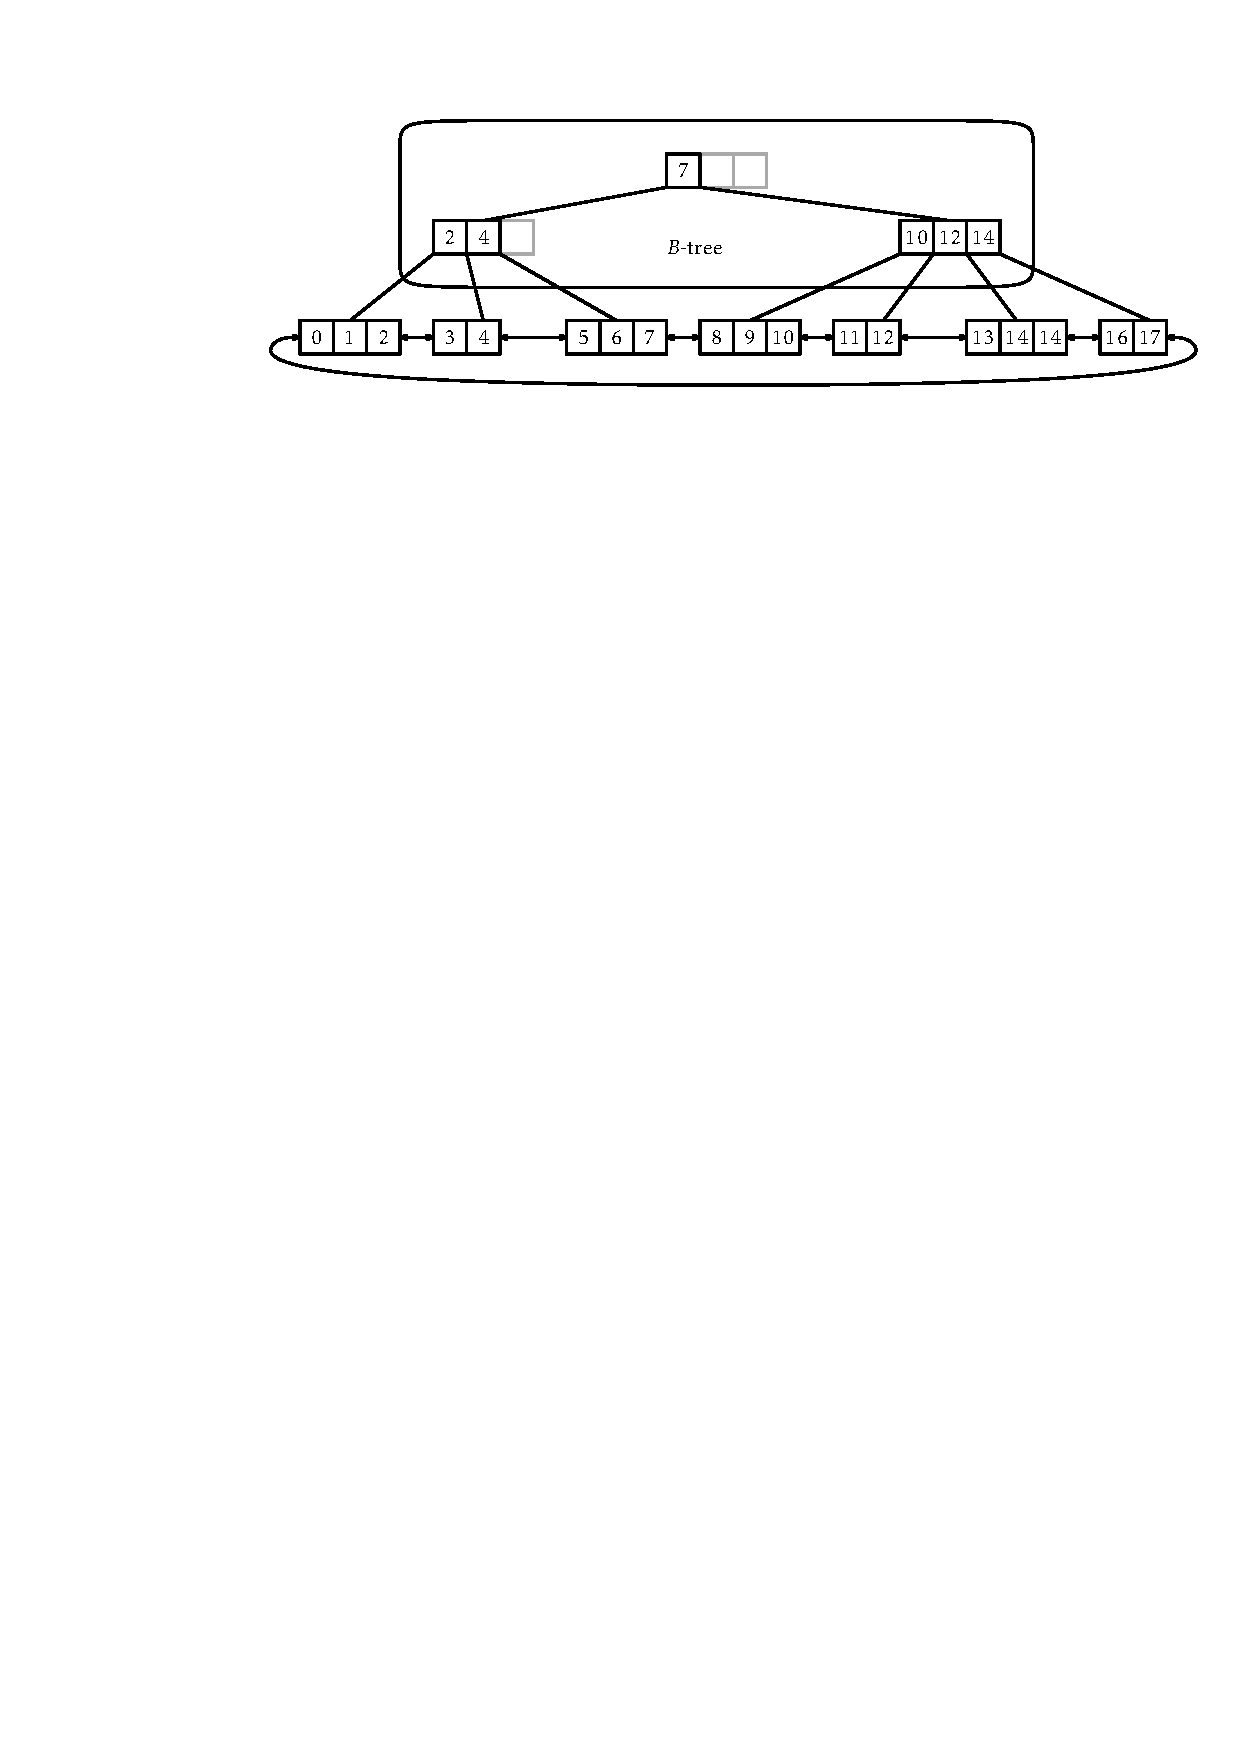
\includegraphics[width=\ScaleIfNeeded]{figs/bplustree}} 
  \caption{Uma árvore $B^+$ é uma árvore $B$ no topo de uma lista duplamente encadeada de blocos.}
  \figlabel{bplustree}
\end{figure}


